\documentclass[11pt,a4paper]{article}
\usepackage[margin=25mm,headheight=15pt]{geometry}
\usepackage[T1]{fontenc}
\usepackage{lmodern,microtype}
% Explicit bundled font maps also support minimally initialized TeX Live installs.
\ifdefined\pdfmapfile
  \pdfmapfile{=lm.map}\pdfmapfile{+cm.map}\pdfmapfile{+symbols.map}
\fi
\usepackage{amsmath,amssymb,amsthm,mathtools}
\usepackage{booktabs,longtable,array,graphicx,xcolor,enumitem,fancyhdr}
\usepackage{listings}
\usepackage[colorlinks=true,linkcolor=blue!45!black,urlcolor=blue!55!black,citecolor=blue!45!black]{hyperref}
\definecolor{ink}{HTML}{16324F}
\definecolor{muted}{HTML}{52616B}
\newcommand{\N}{\mathbb N}
\newcommand{\Z}{\mathbb Z}
\newcommand{\Q}{\mathbb Q}
\newcommand{\R}{\mathbb R}
\newcommand{\ipra}{\ensuremath{\mathsf{iPRA}}}
\newcommand{\PR}{\ensuremath{\mathsf{PR}}}
\newcommand{\norm}[1]{\left\lVert #1\right\rVert}
\newcommand{\dotp}[2]{\left\langle #1,#2\right\rangle}
\newcommand{\epsn}{2^{-n}}
\newcommand{\abs}[1]{\left|#1\right|}
\newcommand{\gap}{\operatorname{Gap}}
\newcommand{\sgn}{\operatorname{sgn}}
\newcommand{\diag}{\operatorname{diag}}
\newcommand{\rank}{\operatorname{rank}}
\newcommand{\tr}{\operatorname{tr}}
\newtheorem{theorem}{Theorem}[section]
\newtheorem{lemma}[theorem]{Lemma}
\newtheorem{proposition}[theorem]{Proposition}
\newtheorem{corollary}[theorem]{Corollary}
\theoremstyle{definition}
\newtheorem{definition}[theorem]{Definition}
\newtheorem{example}[theorem]{Example}
\theoremstyle{remark}
\newtheorem{remark}[theorem]{Remark}
\setlength{\parskip}{4pt}
\setlength{\parindent}{0pt}
\setlength{\emergencystretch}{3em}
\setlist{itemsep=2pt,topsep=4pt}
\pagestyle{fancy}
\fancyhf{}
\fancyhead[L]{\small\color{muted}Analytic geometry in intuitionistic PRA}
\fancyhead[R]{\small\color{muted}Research packet}
\fancyfoot[C]{\thepage}
\renewcommand{\headrulewidth}{0.3pt}
\lstset{basicstyle=\ttfamily\footnotesize,breaklines=true,columns=fullflexible,keepspaces=true,frame=single,rulecolor=\color{gray!25}}
\hypersetup{pdftitle={Analytic geometry in intuitionistic primitive recursive arithmetic},pdfauthor={Research prepared for Vladimir Reshetnikov},pdfsubject={Constructive coordinate geometry, explicit primitive recursive witnesses, and Lean formalization}}
\begin{document}
\begin{titlepage}
\vspace*{14mm}
{\color{ink}\Huge\bfseries Analytic geometry\\[3mm]in intuitionistic\\[3mm]primitive recursive arithmetic\par}
\vspace{12mm}
{\Large Constructive proofs, explicit numerical witnesses,\\ finite-precision contracts, and a Lean completion path\par}
\vspace{14mm}
{\large Prepared for Vladimir Reshetnikov\par}
{\large 22 November 2026\par}
\vspace{14mm}
\begin{abstract}
We develop a broad, explicitly constructive portion of coordinate geometry: affine incidence, metric identities, projections, intersections, conic classification, focal descriptions, quadrics, coordinate transformations, and quantitative tangency. Rational geometric data are encoded by natural numbers. Algebraic lengths and intersection points are supplied by bounded dyadic square-root procedures; analytic coordinate functions are represented by fixed primitive-recursive approximation families. Every division and case distinction is assigned an appropriate domain guard.

The intended arithmetic is first-order intuitionistic primitive recursive arithmetic with quantifier-free induction. No universal primitive-recursive evaluator, arbitrary-real sign oracle, unrestricted choice, or completeness axiom is assumed. The report supplies full mathematical arguments and an explicit translation discipline. It also supplies candidate Lean proofs in ProveIt's actual object-language proof type, together with definitions and remaining formalization obligations. The new Lean source has \textbf{not been compiled in this environment}; executable arithmetic and symbolic checks are separate evidence, not substitutes for formal proofs.
\end{abstract}
\vfill
{\small\color{muted}Repository reference: ProveIt, commit \texttt{bbb85238dac533fc4b7b84a750cca864fe35fed5}.\\
Scope source: \emph{Analytic geometry}, Wikipedia revision 1383468283, and selected relevant immediate outgoing links. Mathematical arguments in this report are developed independently.}
\end{titlepage}
\tableofcontents
\clearpage
\section{Scope, interpretation, and evidence}
\label{sec:scope}

The task is to establish as much of the mathematics in the analytic-geometry article and its relevant immediate links as can be justified constructively in \ipra. There is no finite, canonical maximum: links such as Euclidean space, algebraic geometry, and differential geometry open entire subjects. We therefore give a substantial, reproducible collection concentrated on the article's mathematical spine, and a coverage ledger that identifies the interpretation of each result. Historical and biographical assertions are outside the mathematical task.

Three distinctions govern the work. First, a rational input does not imply a rational output: two rational circles can meet at irrational points. Second, a formula about all real points must be interpreted by a stated representation; natural-number codes do not magically code every classical real. Third, a Lean proof over \texttt{Real} or \texttt{Rat} is not by itself a proof in an embedded first-order theory. The final formal target is a derivation of type \texttt{Prf PRAAx} for a displayed arithmetic sentence.

\subsection{Three kinds of assertion}

\begin{description}[style=nextline]
\item[Exact rational assertions (E).]
Input coordinates, coefficients, and parameters are rational codes. Equality and order are decided by integer arithmetic. Constructed points are rational unless a square-root output is explicitly stated. These assertions translate directly into first-order arithmetic.
\item[Constructed algebraic outputs (A).]
A rational problem produces finitely many explicit expressions using rational operations and nonnegative square roots. Each expression has a primitive-recursive approximation program with a proved error bound. This is sufficient for the intersections and canonical-form witnesses below; a general real-algebraic-number decision procedure is not silently invoked.
\item[Represented-real schemas (R).]
For each \emph{fixed} primitive-recursive family of coordinate names, with supplied bounds and any required apartness data, we prove an arithmetic statement about all requested precisions. The family is fixed outside the formula; its numerical parameters and precision indices are quantified inside the formula. Universal quantification over an arbitrary function space is never introduced.
\end{description}

When an elementary identity is written with real-looking coordinates, its E reading is immediate. Its R reading uses the quantitative translation of Section~\ref{sec:foundations}; a branching assertion does \emph{not} acquire an R reading unless all branch information is supplied. Exact comparison of the resulting names is not an operation of this representation.

\subsection{What was reused from ProveIt}

The repository was inspected at the commit printed on the title page. Its directory README explicitly separates checked derivation libraries from delivered research packets~\cite{repo-main}. We inspected the concrete modules
\path{Geometry/PlaneMetric.lean} and
\path{Geometry/IsoperimetricDyadicSquareRoot.lean} under
\path{Derivations/Lean/IPRADerivations/}~\cite{repo-metric,repo-sqrt}.
The first contains the actual object-iPRA Gram and parallelogram identities. The second exposes the bracket, maximality, source bound, and program equations for a dyadic square root. These are unusually close to the present needs.

We also inspected the planar Euclidean-geometry and Euler--Rodrigues packet READMEs~\cite{repo-plane-packet,repo-rotation-packet}. They motivate useful interfaces and identify existing work, but their general claims are not imported as axioms. In particular, this report does not rely on a completed quantifier-elimination theorem for algebraic numbers. The elementary arguments needed here are supplied below. The repository's published build status was not independently replayed in this environment.

\subsection{Corrections and necessary qualifications}

Several informal textbook sentences require extra conditions. A negative conic discriminant does not guarantee a nonempty ellipse: $x^2+y^2+1=0$ has no real point. Two conics may share a component and then have infinitely many common points. The expression $\arctan(y/x)$ is neither defined on the vertical axis nor a correct global angular coordinate. A tangent may cross its curve, and a singular point need not have a unique tangent. All corresponding positive statements in this packet include the relevant conditions; these are mathematical distinctions, not merely numerical implementation choices.

The source ledger uses the Wikipedia pages as a topic inventory~\cite{wiki-main}. The proofs and numerical bounds are original developments for this packet. The primary-source comparison for standard plane and tangent equations is Paul Dawkins's course material~\cite{dawkins}; ProveIt's source is the primary reference for its own formal interface.

\section{The arithmetic foundation and its real-name boundary}
\label{sec:foundations}

\subsection{The exact theory and numerical codes}

We use intuitionistic first-order logic with equality. Its nonlogical symbols are $0,S$ and a function symbol for each specified primitive-recursive definition. The nonlogical axioms are the defining equations, $Sx\ne0$, successor injectivity, and, for every quantifier-free formula $A(n,\mathbf a)$, the induction axiom
\[
 \bigl(A(0,\mathbf a)\wedge
   \forall n\,[A(n,\mathbf a)\to A(Sn,\mathbf a)]\bigr)
       \longrightarrow \forall n\,A(n,\mathbf a).
\]
The logical rules are the ordinary intuitionistic introduction and elimination rules for $\wedge,\vee,\to,\forall,\exists,\bot$, together with equality substitution. No induction instance whose matrix contains an unbounded quantifier is used.

The following concrete coding choices suffice. Encode the integer $m\ge0$ by $2m$, and $-(m+1)$ by $2m+1$. A rational code is a pair $(z,d)$ with $d\ge1$, representing $\operatorname{int}(z)/d$; unreduced fractions are allowed. Natural-number pairs can be encoded by
\[
 \langle a,b\rangle=(a+b)^2+a.
\]
This is injective: for $s=a+b$, its value lies in $[s^2,s^2+s]$, and these intervals are disjoint. Both components can be recovered by a bounded double search with bound equal to the code. Codes outside the image decode to $(0,0)$. A rational denominator is stored as $d-1$, so every decoded rational has a positive denominator. A list is its length together with nested pair codes; its entries are recovered by iteration for the recorded length. Invalid structure is assigned a fixed default.

For $a/b,c/d$ with $b,d>0$, use
\[
 \frac ab+\frac cd=\frac{ad+bc}{bd},\quad
 \frac ab\frac cd=\frac{ac}{bd},\quad
 \frac ab\le\frac cd\ \Longleftrightarrow\ ad\le bc.
\]
The reciprocal is $\sgn(a)b/|a|$ when $a\ne0$, and is totalized as $0$ when $a=0$. Theorems involving a reciprocal carry the nonzero guard. Integer signs, absolute values, comparisons, quotients and remainders are all primitive recursive; quotient, for example, is the greatest $q\le a$ with $bq\le a$ when $b>0$.

\begin{proposition}[Coded ordered-rational arithmetic]\label{found:rat}
The above operations are primitive recursive. The ordered-field identities and order rules for rational values are provable in \ipra, with the indicated positive-denominator and nonzero guards. Equality of codes is replaced, where necessary, by equality of represented rational values.
\end{proposition}
\begin{proof}
Parity, truncated subtraction, and bounded maximum are defined by recursion on natural numbers. Their correctness is proved by quantifier-free induction on their counters. Thus every displayed rational operation is a composition of primitive-recursive functions. To verify equality, cross-multiply positive denominators. Associativity of addition becomes the integer identity
$(ad+bc)f+ebd=adf+bcf+ebd$ after common denominators are inserted; multiplication, distributivity and the guarded inverse law are equally direct. The natural semiring laws follow by induction from the defining equations for addition and multiplication. Signed-integer laws follow by representing an integer as a difference of naturals and cross-adding the two sides; subtraction introduces no new induction principle. Order transitivity and preservation under addition follow from the corresponding natural-number order laws after positive denominator multiplication. A positive product has positive factors' signs, so denominator clearing preserves the direction of each comparison. Every proof has a fixed, finite algebraic form. No choice of a canonical fraction is needed.
\end{proof}

\begin{lemma}[Finite loops and bounded formulas]\label{found:loops}
A loop with a primitive-recursive number of iterations, primitive-recursive state update, and a quantifier-free invariant admits its usual invariant proof in \ipra. A bounded collection of decidable rational tests can be used in that invariant.
\end{lemma}
\begin{proof}
Define the state after $j$ iterations by primitive recursion, freeze it after the specified bound, and apply quantifier-free induction to the coded invariant at $j$. A conjunction of tests indexed by $i<b$ is the Boolean product of their characteristic values; disjunction is computed by a Boolean maximum. Their equivalence to the corresponding bounded formulas is proved by induction on $b$. Consequently a loop invariant with a bounded list of rational equalities or inequalities is an abbreviation for a quantifier-free formula. This is a derived use of bounded formulas, not stronger induction.
\end{proof}

Polynomial expressions in a fixed finite number of variables may be stored as finite coefficient--exponent lists. Evaluation is a bounded sum of products of powers, hence is uniformly primitive recursive even when degree is input data. This restricted evaluator is entirely different from an evaluator for arbitrary primitive-recursive programs.

\subsection{A square root with an actual stopping bound}

For $a\ge0$, $b\ge1$, and $n\in\N$, put $H=2^n$ and
\[
 B=(a+1)H,\qquad
 j(a,b,n)=\max\{j\le B:b j^2\le aH^2\},\qquad
 s_n(a/b)=j(a,b,n)/H.
\]
The bounded set contains zero. This formula is a primitive-recursive search, whether implemented as a scan or by integer square root after division.

\begin{theorem}[Dyadic square-root bracket]\label{found:sqrt}
For every $a\ge0,b\ge1,n\in\N$,
\[
 b j^2\le a4^n<b(j+1)^2,
 \qquad s_n^2\le a/b<(s_n+2^{-n})^2.
\]
Moreover $j<B$, $s_n\le s_{n+1}<s_n+2^{-n}$, and the nested intervals
$[s_n,s_n+2^{-n}]$ give a primitive-recursive name for the unique nonnegative square root of $a/b$.
\end{theorem}
\begin{proof}
The loop that maintains the greatest acceptable candidate has the quantifier-free invariant ``the current candidate is acceptable and every tested larger candidate is unacceptable.'' Its bounded universal clause is handled by Lemma~\ref{found:loops}. Since $(a+1)^2>a$ and $b\ge1$, $bB^2>aH^2$, so the maximum is strictly below $B$. The next integer is therefore tested and fails, proving the bracket.

At precision $n+1$, the inequalities for $2j$ and $2j+2$ show that the next maximum is either $2j$ or $2j+1$. This proves the nesting and the distance estimate. For any two nonnegative numbers whose squares equal $a/b$, the elementary identity
$(u-v)(u+v)=u^2-v^2$ shows uniqueness: on rational enclosing intervals, a positive separation of $u,v$ would imply a positive separation of their squares. An entirely finite version is given in the next lemma. Thus the name is specified by its brackets without assuming a completeness axiom in the object theory. The word ``square root'' is shorthand for these arithmetic contracts.
\end{proof}

\begin{lemma}[Square-root order and a uniform modulus]\label{found:holder}
For nonnegative rational $u,v$, their constructed roots obey monotonicity and
\[
 |\sqrt u-\sqrt v|^2\le |u-v|.
\]
More explicitly, if $h=2^{-m}$ and $B$ is a common rational upper bound for the two lower approximations, then
\[
 |s_m(u)-s_m(v)|^2\le |u-v|+2Bh+h^2.
\]
These statements have finite-precision versions provable in \ipra. In particular the square-root operation needs no positive lower bound at zero.
\end{lemma}
\begin{proof}
For nonnegative rational $p\ge q$, one has
$(p-q)^2\le(p-q)(p+q)=p^2-q^2$. Also $p^2\le q^2$ and $p,q\ge0$ imply $p\le q$: if $p>q$, then $(p-q)(p+q)>0$. Apply these rational inequalities to the lower and upper endpoints in Theorem~\ref{found:sqrt}. If $p=s_m(u)\ge q=s_m(v)$, then
\[
 (p-q)^2\le p^2-q^2\le u-v+2qh+h^2
             \le |u-v|+2Bh+h^2;
\]
the other rational case is symmetric. Their widths are $2^{-m}$, and these explicit error terms vanish at a chosen finer precision. More explicitly, if a fixed rational observation inequality fails by $\eta>0$, choose $m$ with its computed error bound less than $\eta$; bounded search up to the numerator and denominator data finds such an $m$. This contradicts the finite rational endpoint inequality. This argument is intuitionistically valid because only a rational comparison is split into cases. It also proves uniqueness of a nonnegative root name. No trichotomy on real names is involved.
\end{proof}

\subsection{Fixed primitive-recursive real families}

\begin{definition}[Names, bounds, and apartness]\label{found:names}
A name is a \emph{fixed} primitive-recursive rational-valued function
$X(\mathbf a,n)$, with numerical parameters $\mathbf a$, satisfying
\[
 \forall m,n\quad |X(\mathbf a,m)-X(\mathbf a,n)|
                 \le 2^{-m}+2^{-n}.
\]
We write $x$ for this family in mathematical prose. A bound $M$ supplies
$|X(\mathbf a,n)|\le M+2^{-n}$. Nonnegativity means
$X(\mathbf a,n)\ge-2^{-n}$ for all $n$. An apartness bound $k$ supplies
\[
 |X(\mathbf a,n)|\ge 2^{-k}-2^{-n}\quad\hbox{for all }n.
\]
Equality and order of names are propositions about all precisions, never Boolean tests. For example, $x=y$ can be expressed by
$|X(m)-Y(n)|\le2^{-m}+2^{-n}$ for all $m,n$; $x\le y$ is expressed by
$X(m)\le Y(n)+2^{-m}+2^{-n}$ for all $m,n$.
\end{definition}

All these formulas are first-order arithmetic formulas after the fixed programs are expanded. Their universal quantifiers do not occur in induction matrices. Pointwise arguments are carried out at a requested precision, with the finitely many required instances of the hypotheses. Displaying an ``exact'' identity between names means all of these finite rational conclusions, not an equality test on the names' program codes.

Let $\ell(B)$, for an integer $B\ge1$, be the least $j\le B$ with $B\le2^j$; this is a bounded primitive-recursive search. For rational bounds use their natural-number ceilings first.

\begin{theorem}[Arithmetic on names with explicit precision]\label{found:operations}
Fixed PR names are closed under addition, subtraction, multiplication, absolute value, and nonnegative square root. They are closed under reciprocal when an apartness bound is supplied. The constructions have primitive-recursive precision schedules and their defining contracts are provable in \ipra.
\end{theorem}
\begin{proof}
For readability write an approximation error as $\varepsilon=2^{-m}$; all estimates below are rational endpoint estimates, so the same proof gives the formulas of Definition~\ref{found:names}. For addition query each input at $m=n+2$; the combined error is at most $2^{-n-1}$. Absolute value is $1$-Lipschitz on rational numbers.

If $|x|,|y|\le M$ and $|p-x|,|q-y|\le\varepsilon\le1$, then
\[
 |pq-xy|\le |p|\,|q-y|+|y|\,|p-x|
             \le(2M+1)\varepsilon.
\]
Take $m=n+\ell(2M+3)+2$. This gives slack for converting one-stage estimates to the two-index name condition.

For a reciprocal put $\delta=2^{-k}$. At $m\ge k+2$, the rational observation has absolute value at least $\delta/2$. The identity
\[
 \left|\frac1p-\frac1x\right|
   =\frac{|p-x|}{|p|\,|x|}
   \le 2\delta^{-2}|p-x|
\]
is a guarded rational identity when endpoint bounds are used. Taking
$m=n+2k+3$ gives error at most $2^{-n-2}$. The program tests whether its sampled rational is zero and returns zero there, so it remains total off the promised domain. The apartness hypothesis proves that this default branch is not used on the domain.

For square root, query a nonnegative input at $m=2n+6$, replace a negative observation by zero, and compute its rational square root at precision $n+2$ by Theorem~\ref{found:sqrt}. Clipping changes neither the nonnegative target nor its error bound. Lemma~\ref{found:holder} bounds the input error in the root by $2^{-n-3}$; the final dyadic bracket contributes at most $2^{-n-2}$. Their sum is less than $2^{-n}$. Every search and index in this construction is primitive recursive.

To remove the suggestive occurrences of $x$ in these estimates, replace it throughout by an observation at a common later index $r$, use the Cauchy and bound hypotheses at $(m,r)$, and leave the extra $2^{-r}$ terms visible. For each target rational inequality, choose $r$ so their explicit coefficient times $2^{-r}$ fits the reserved slack. For exact weak inequalities at a boundary, the rational failure argument of Lemma~\ref{found:holder} applies. This proves the displayed first-order contracts without appealing to real completeness.
\end{proof}

\begin{proposition}[Finite algebra and quantified name identities]\label{found:transfer}
Every fixed polynomial identity established by ring algebra transfers to fixed PR names. A fixed rational expression transfers when every denominator has a supplied apartness bound. Rational coefficient inequalities, a priori magnitude bounds, and square-root contracts can be composed with these transfers. This is a schema for the particular finite expressions used below, not a truth-reflection principle for arbitrary formulas.
\end{proposition}
\begin{proof}
For a polynomial $P=\sum_\alpha c_\alpha X^\alpha$ on $|X_i|\le M$ and observations within $\varepsilon\le1$, telescope one factor at a time in each monomial. The resulting explicit bound is
\[
 |P(p)-P(x)|\le L_P(M)\varepsilon,\qquad
 L_P(M)=\sum_\alpha |c_\alpha|\,|\alpha|(M+1)^{|\alpha|}.
\]
Here $|\alpha|$ is the total degree, and the exponent-zero case contributes zero. If $P-Q$ is a polynomial identity, its value on rational observations is exactly zero by Proposition~\ref{found:rat}; the two Lipschitz errors bound the residual. Choose an observation precision exceeding the requested precision by
$\ell(\lceil L_P+L_Q\rceil+1)+3$. Reciprocal and root nodes use Theorem~\ref{found:operations}. Induct on the \emph{finite expression tree in the metatheory}; for each expression this supplies a particular first-order proof. Variable finite coefficient lists can instead use Lemma~\ref{found:loops}. This reasoning never asserts the soundness of all iPRA proofs inside iPRA.
\end{proof}

\subsection{What cannot be hidden in a real-number branch}

\begin{proposition}[No uniform zero test for all these names]\label{found:no-zero-test}
There is no total computable algorithm that, from the description of every fixed PR Cauchy name with the above modulus, always decides whether its value is zero. Consequently a rational classification algorithm below must not be silently advertised as an arbitrary-real classification algorithm.
\end{proposition}
\begin{proof}
For a machine code $e$, simulate it for $n$ steps. If it first halts at step $t\le n$, output $X_e(n)=2^{-t}$; otherwise output zero. Bounded simulation is primitive recursive, and this family satisfies the stated modulus: the only difference between observations before and after a halt at $t$ is $2^{-t}$, which is smaller than $2^{-n}$ at every earlier stage $n<t$. The limiting value is zero exactly when that machine never halts. A total zero test would therefore decide halting. For completeness, a halting decider leads to the program which, on its own code, loops when the decider says it halts and halts when the decider says it loops. Either answer contradicts the specified behavior. This is an external impossibility argument about algorithms; it is not presented as a new internal consistency theorem of \ipra.
\end{proof}

This obstruction leaves all positive constructions intact. Rational determinant signs are decidable, a supplied nonzero gap permits inversion of a name, and a precision request permits certified approximation near a boundary. It only prevents us from replacing those hypotheses by an unstated total oracle.

\subsection{A uniform audit rule for the later proofs}

For each proof below, encode its input tuple as a natural number; expand rational arithmetic as above; totalize every guarded division; unfold its finite sum or bounded search; and use quantifier-free induction only on that explicit loop. A fixed-dimensional determinant computation has no unbounded search. For a name assertion, first fix its PR input families, quantify only their numerical parameters, and prove the requested observation formula with the explicit demand schedule. This rule is used together with the particular identities and bounds proved in each chapter. It is not a license to import an arbitrary classical theorem merely because its conclusion looks computational.

\section{Affine and metric coordinate geometry}
\label{sec:affine-metric}

This chapter treats points and vectors in dimensions two and three. Unless
explicitly stated otherwise their coordinates, the coefficients of equations,
and construction parameters are rational. Thus every equality test and every
sign case below is a test of integers after multiplication by positive
denominators. Lengths and the square roots occurring in intersection formulas
are interpreted by the fixed primitive recursive real names constructed in the
foundational chapter. The assertions extend to fixed families of such names
when the required denominator bounds and sign certificates are supplied;
they do not assert a decision procedure for equality of arbitrary real names.

Write
\[
 \langle u,v\rangle=\sum_{i=1}^{d}u_iv_i,\qquad
 S(u)=\langle u,u\rangle,\qquad |u|=\sqrt{S(u)},\qquad d\in\{2,3\}.
\]
For planar vectors set
\[
 J(u_1,u_2)=(-u_2,u_1),\qquad [u,v]=u_1v_2-u_2v_1.
\]
A nonzero rational vector has strictly positive squared length: one of its
finitely many rational coordinates is nonzero, its square is positive, and
the other squares are nonnegative. Every reciprocal of a squared length
used below is therefore guarded by a decidable, explicitly stated condition.
In particular, no argument obtains a reciprocal from a mere double negation
of nonzeroness.

\subsection{Incidence and affine constructions}

\begin{theorem}[Equivalent equations of a line, and the line through two points]
\label{geo:line}
Let $P\in\Q^2$ and $u\in\Q^2$ with $u\ne0$. Then
\[
 X=P+tu\quad\Longleftrightarrow\quad [u,X-P]=0
 \quad\Longleftrightarrow\quad \langle Ju,X-P\rangle=0.
\]
Here the existential parameter $t$ is uniquely determined and rational for
rational $X$. Consequently two distinct rational points determine a unique
line, and every equation $ax+by=c$ with $(a,b)\ne(0,0)$ describes a line.
\end{theorem}
\begin{proof}
Substitution proves both implications from the parametric equation. Conversely,
if $u_1\ne0$, set $t=(X_1-P_1)/u_1$. The determinant equation says
$u_1(X_2-P_2)=u_2(X_1-P_1)$, so $X_2-P_2=tu_2$.
If $u_1=0$, then $u_2\ne0$, the determinant equation gives $X_1=P_1$,
and $t=(X_2-P_2)/u_2$ works. The same nonzero coordinate proves uniqueness.
For distinct $P,Q$, take $u=Q-P$. A line containing $P$ and $Q$ has a
direction proportional to $u$, so its point set agrees with this one.
Finally, for $n=(a,b)\ne0$, the rational point
$P=(c/S(n))n$ satisfies $\langle n,P\rangle=c$ and the nonzero direction
$Jn$ is perpendicular to $n$. The equivalence already proved gives the
required line. All branches and quotients have displayed rational guards.
\end{proof}

\begin{theorem}[Slope, intercepts, parallelism, and perpendicularity]
\label{geo:slope}
For $(a,b)\ne(0,0)$, the line $ax+by=c$ has slope-intercept equation
$y=mx+k$ with $m=-a/b$ and $k=c/b$ when $b\ne0$; when $b=0$ it is the
vertical line $x=c/a$. Its intersections with the axes are obtained by
setting the other coordinate equal to zero, with the zero-coefficient case
giving either the whole axis or no point. Two nonvertical lines with slopes
$m,m'$ have parallel directions exactly when $m=m'$, and perpendicular
directions exactly when $mm'=-1$.
\end{theorem}
\begin{proof}
Solving the equation for $y$, or for $x$ if $b=0$, proves the first assertion.
For the $x$-axis the remaining equation is $ax=c$: if $a\ne0$ the unique
intercept is $(c/a,0)$; if $a=0$ its truth is the decidable test $c=0$.
The $y$-axis is identical with the roles reversed. Directions of the two
nonvertical lines can be chosen as $(1,m)$ and $(1,m')$. Their determinant
is $m'-m$ and their dot product is $1+mm'$, proving the last assertions.
The treatment of vertical lines explains why a slope alone cannot represent
every line and why the perpendicular-slope formula requires its stated domain.
\end{proof}

\begin{theorem}[Complete intersection classification of two rational lines]
\label{geo:two-lines}
Consider $ax+by=c$ and $a'x+b'y=c'$, with both normal vectors nonzero, and
put $\Delta=ab'-ba'$. If $\Delta\ne0$, their unique intersection is
\[
 x=\frac{cb'-bc'}{\Delta},\qquad
 y=\frac{ac'-ca'}{\Delta}.
\]
If $\Delta=0$, the lines coincide precisely when
$ac'=a'c$ and $bc'=b'c$; otherwise they are disjoint.
\end{theorem}
\begin{proof}
Multiplying the equations respectively by $b',b$ and subtracting gives
$\Delta x=cb'-bc'$. The analogous elimination gives
$\Delta y=ac'-ca'$. This proves necessity and uniqueness when the determinant
is nonzero, and direct substitution proves existence.
If the determinant vanishes, choose a nonzero coordinate of $(a,b)$.
For example, when $a\ne0$, the determinant equation gives
$(a',b')=\lambda(a,b)$ for $\lambda=a'/a$.
Because the second normal is nonzero, $\lambda\ne0$.
The two equations are then consistent exactly when $c'=\lambda c$,
equivalently $ac'=a'c$. The additional displayed equality follows from it.
The branch $a=0$ uses $b\ne0$ and is identical. An inconsistent proportional
pair cannot have a common point because substitution would force the failed
constant equality. This is a finite rational case split, including coincidence.
\end{proof}

\begin{theorem}[Determinant, collinearity, and triangle area]
\label{geo:area}
For $A,B,C\in\Q^2$, define the signed area
\[
 \mathcal A(A,B,C)=\tfrac12[B-A,C-A].
\]
It is translation invariant, changes sign on interchanging two vertices,
and is zero exactly when the three points are collinear, allowing coincident
points. Its absolute value is one half of base length times perpendicular
height. For every $P$ one has
\[
 \mathcal A(A,B,C)=\mathcal A(P,B,C)+\mathcal A(A,P,C)+\mathcal A(A,B,P).
\]
\end{theorem}
\begin{proof}
Translation cancels in both differences; exchanging $B,C$ reverses the
determinant. Exchanging $A,B$ gives
$[A-B,C-B]=[-(B-A),(C-A)-(B-A)]=-[B-A,C-A]$.
If $A\ne B$, the zero determinant is exactly the line criterion of
Theorem~\ref{geo:line}. If $A=B$, any line through $A,C$ works, and if all
three coincide the horizontal line through them works.
For nonzero base $u=B-A$, decompose $v=C-A$ as
\[
 v=\frac{\langle u,v\rangle}{S(u)}u+
       \frac{[u,v]}{S(u)}Ju.
\]
The identity follows coordinatewise; the second summand is perpendicular
to the base and has length $|[u,v]|/|u|$. Hence half base times height is
$|[u,v]|/2$. A zero base gives zero area directly.
Finally, expand every determinant in the last displayed equation using
$[X-Y,Z-Y]=[X,Z]-[X,Y]-[Y,Z]$; all terms containing $P$ cancel.
This also verifies finite additivity of oriented triangle area without a
topological argument about the inside of a curve.
\end{proof}

\begin{theorem}[Section formula, midpoint, and segment inequalities]
\label{geo:section}
Let $P,Q\in\Q^d$, $P\ne Q$, and $t\in\Q$. The point
$R=(1-t)P+tQ$ is on their line and is on the closed segment precisely when
$0\le t\le1$. In that case
$|R-P|=t|Q-P|$ and $|Q-R|=(1-t)|Q-P|$.
For positive rationals $m,n$, the unique point on the segment with
$|R-P|:|Q-R|=m:n$ is
\[
 R=\frac{nP+mQ}{m+n}.
\]
The midpoint $M=(P+Q)/2$ satisfies, for every $X$,
\[
 S(X-P)+S(X-Q)=2S(X-M)+\tfrac12 S(P-Q).
\]
\end{theorem}
\begin{proof}
The segment is defined parametrically by $0\le t\le1$, and the uniqueness
of the line parameter makes this definition unambiguous. The differences
are $t(Q-P)$ and $(1-t)(Q-P)$, whose lengths have the displayed values by
nonnegativity of $t,1-t$. The ratio equation reduces, after cancelling the
positive base length, to $nt=m(1-t)$, whose unique solution is
$t=m/(m+n)$. For the last identity set $a=X-M$ and $b=(Q-P)/2$.
The left side is $S(a+b)+S(a-b)=2S(a)+2S(b)$, because the two cross terms
cancel. This proves the midpoint identity by a finite polynomial calculation.
\end{proof}

\begin{theorem}[Barycentric coordinates and concurrence of medians]
\label{geo:centroid}
If $A,B,C\in\Q^2$ are noncollinear, every rational point $X$ has unique
rational barycentric coordinates $\alpha,\beta,\gamma$ with
\[
 \alpha+\beta+\gamma=1,\qquad X=\alpha A+\beta B+\gamma C.
\]
They are
\[
 \alpha=\frac{\mathcal A(X,B,C)}{\mathcal A(A,B,C)},\quad
 \beta=\frac{\mathcal A(A,X,C)}{\mathcal A(A,B,C)},\quad
 \gamma=\frac{\mathcal A(A,B,X)}{\mathcal A(A,B,C)}.
\]
The three medians meet uniquely at $G=(A+B+C)/3$, which divides each median
in the ratio $2:1$ measured from its vertex.
\end{theorem}
\begin{proof}
Write $u=B-A$, $v=C-A$. The system $X-A=\beta u+\gamma v$ has a unique
solution because $[u,v]\ne0$. Taking determinants with $v$ and with $u$
gives $\beta=[X-A,v]/[u,v]$ and $\gamma=[u,X-A]/[u,v]$.
Set $\alpha=1-\beta-\gamma$; the area-addition identity proves the formula
for $\alpha$. If $M=(B+C)/2$, then
$G=A+\frac23(M-A)$, so the section formula proves the claimed ratio and
incidence. A point on the median from $A$ has $\beta=\gamma$; a point on
the median from $B$ has $\alpha=\gamma$. Their unique common solution is
$\alpha=\beta=\gamma=1/3$. Thus concurrency and uniqueness are both explicit.
\end{proof}

\begin{theorem}[Affine changes of coordinates]
\label{geo:affine}
Let $T(X)=MX+b$ on $\Q^2$. It preserves affine combinations whose coefficients
sum to one. If $\det M\ne0$, it is bijective, maps lines to lines, preserves
the parameter of every section of a line, and obeys
\[
 [Mu,Mv]=(\det M)[u,v],\qquad
 \mathcal A(TA,TB,TC)=(\det M)\mathcal A(A,B,C).
\]
For a locus $F(X)=0$, its image is described by
$F(M^{-1}(Y-b))=0$.
\end{theorem}
\begin{proof}
Linearity gives
$T(\sum_i\lambda_iX_i)=\sum_i\lambda_iT(X_i)$ when $\sum_i\lambda_i=1$.
For $M=\left(\begin{smallmatrix}a&b_0\\c&d\end{smallmatrix}\right)$,
expansion gives
\[
 (au_1+b_0u_2)(cv_1+dv_2)-(cu_1+du_2)(av_1+b_0v_2)
 =(ad-b_0c)(u_1v_2-u_2v_1).
\]
The inverse matrix is
$(ad-b_0c)^{-1}\left(\begin{smallmatrix}d&-b_0\\-c&a\end{smallmatrix}\right)$,
verified by multiplication. Thus a nonzero direction stays nonzero, and
$T(P+tu)=T(P)+tMu$ proves the assertions about lines and sections.
The area formula follows from the determinant identity. Finally
$Y=T(X)$ is equivalent to $X=M^{-1}(Y-b)$, proving both directions of
the locus transformation. The inverse substitution is essential: substituting
the forward map into $F$ would describe its inverse image.
\end{proof}

\subsection{Inner products, distances, projections, and isometries}

\begin{theorem}[Lagrange's sum-of-squares identity]
\label{geo:lagrange}
In dimensions two and three,
\[
 S(u)S(v)-\langle u,v\rangle^2
 =\sum_{1\le i<j\le d}(u_iv_j-u_jv_i)^2.
\]
In the plane the right side is $[u,v]^2$. It vanishes precisely when $u,v$
are linearly dependent, including the case where one vector is zero.
\end{theorem}
\begin{proof}
Expand the product as
$\sum_i u_i^2v_i^2+\sum_{i<j}(u_i^2v_j^2+u_j^2v_i^2)$.
The square of the dot product is
$\sum_i u_i^2v_i^2+2\sum_{i<j}u_iu_jv_iv_j$.
Subtracting leaves exactly the displayed squares. If they all vanish and
$u\ne0$, choose $k$ with $u_k\ne0$. Each equation
$u_kv_j-u_jv_k=0$ gives $v_j=(v_k/u_k)u_j$, proving dependence.
If $u=0$, dependence is immediate. Conversely proportional vectors make
every minor vanish. A finite sum of nonnegative rational squares is zero
only if each square is zero, a fact proved by rational order and the finite
number of summands.
\end{proof}

\begin{theorem}[Cauchy--Schwarz and its equality condition]
\label{geo:cauchy}
For $u,v\in\Q^d$,
\[
 |\langle u,v\rangle|\le |u||v|.
\]
Equality holds exactly when the vectors are linearly dependent. For nonzero
vectors the normalized dot product lies between $-1$ and $1$.
\end{theorem}
\begin{proof}
The sum of squares in Theorem~\ref{geo:lagrange} is nonnegative, so
$\langle u,v\rangle^2\le S(u)S(v)$. Both sides of the desired inequality
are nonnegative; comparison of their squares proves it, using monotonicity
of the nonnegative square root. Equality is equivalent to the vanishing
of the difference of those squares, hence to linear dependence by the same
theorem. If both squared lengths are positive, their product has a positive
square root, so division gives the final assertion. For rational inputs this
positive denominator has an explicit rational lower bound, obtainable from
the input numerators and denominators or the square-root construction.
\end{proof}

\begin{theorem}[Pythagoras, parallelogram identity, and polarization]
\label{geo:pythagoras}
The identities
\[
 S(u+v)=S(u)+2\langle u,v\rangle+S(v),\qquad
 S(u+v)+S(u-v)=2S(u)+2S(v)
\]
hold in dimensions two and three. In particular,
$S(u+v)=S(u)+S(v)$ exactly when $\langle u,v\rangle=0$.
Moreover
\[
 \langle u,v\rangle=\tfrac14\bigl(S(u+v)-S(u-v)\bigr).
\]
\end{theorem}
\begin{proof}
For each coordinate,
$(u_i+v_i)^2=u_i^2+2u_iv_i+v_i^2$.
Summation proves the first identity. Replacing $v$ by $-v$ and adding cancels
the dot products; subtracting instead yields four times the dot product.
The Pythagorean equivalence follows by subtracting $S(u)+S(v)$ and using
the nonzero rational constant $2$. Thus the usual geometric right-angle
criterion, defined by a zero inner product, is equivalent to the squared
length identity; no angle-selection operation is needed.
\end{proof}

\begin{theorem}[The Euclidean distance is a metric]
\label{geo:metric}
Define $d(P,Q)=\sqrt{\sum_i(P_i-Q_i)^2}$. It is nonnegative and symmetric,
equals zero exactly when $P=Q$, and satisfies
\[
 d(P,R)\le d(P,Q)+d(Q,R).
\]
For a nonnegative rational $a$, $d(aP,aQ)=a\,d(P,Q)$.
\end{theorem}
\begin{proof}
Nonnegativity is part of the square-root specification. Reversing each
difference leaves its square unchanged, proving symmetry. If the distance
is zero, its square is zero, and each nonnegative coordinate square is zero;
therefore all coordinate differences vanish. The converse is immediate.
For the triangle inequality put $u=P-Q$ and $v=Q-R$. By the preceding
theorems,
\[
 S(u+v)=S(u)+2\langle u,v\rangle+S(v)
 \le S(u)+2|u||v|+S(v)=(|u|+|v|)^2.
\]
Taking nonnegative square roots gives $|u+v|\le|u|+|v|$.
Finally $S(a(P-Q))=a^2S(P-Q)$, and $a|P-Q|$ is the unique nonnegative
square root of that value. Every appeal to square roots is an inequality
or equality of the represented values; no branching on their equality occurs.
\end{proof}

\begin{theorem}[Cosine law and an algebraic encoding of planar angles]
\label{geo:cosine}
For a triangle with side vectors $u,v$ at one vertex and nonzero adjacent
lengths $a=|u|$, $b=|v|$, set
$c_\theta=\langle u,v\rangle/(ab)$. Then
\[
 |u-v|^2=a^2+b^2-2ab c_\theta.
\]
In the plane, set also $s_\theta=[u,v]/(ab)$. Then
$c_\theta^2+s_\theta^2=1$. These two numbers encode an oriented angle
without choosing an inverse trigonometric branch. For nonvertical directions
$(1,m),(1,m')$, when $1+mm'\ne0$, the corresponding sine-to-cosine ratio is
\[
 \frac{s_\theta}{c_\theta}=\frac{m'-m}{1+mm'}.
\]
\end{theorem}
\begin{proof}
The cosine law is the expansion of $S(u-v)$ followed by the definition of
$c_\theta$. The planar Lagrange identity gives
$\langle u,v\rangle^2+[u,v]^2=S(u)S(v)=a^2b^2$;
division proves the unit-circle equation. The dot product of the two slope
directions is $1+mm'$ and their determinant is $m'-m$, so their common
normalizing factor cancels in the displayed quotient. The nonzero-denominator
condition excludes a right angle, where this quotient has no finite value.
The normalized pair remains defined there and also records the quadrant
information lost by an unqualified arctangent of a slope.
\end{proof}

\begin{theorem}[Projection onto a line and its minimum-distance property]
\label{geo:projection}
Let $L=\{P+tu:t\in\Q\}$ with $u\ne0$, and let $X\in\Q^d$.
The perpendicular foot is
\[
 H=P+\frac{\langle X-P,u\rangle}{S(u)}u.
\]
It is the unique point of the line minimizing squared distance to $X$, since
for every parameter $t$,
\[
 S\bigl(X-(P+tu)\bigr)
 =S(X-H)+S(u)\left(t-\frac{\langle X-P,u\rangle}{S(u)}\right)^2.
\]
In the plane,
$S(X-H)=[u,X-P]^2/S(u)$; in three dimensions it is
$S(X-P)-\langle X-P,u\rangle^2/S(u)$.
\end{theorem}
\begin{proof}
The chosen coefficient makes $\langle X-H,u\rangle=0$.
Write $X-(P+tu)=(X-H)+(t_0-t)u$, where $t_0$ is that coefficient.
Pythagoras gives the displayed decomposition. Its second term is nonnegative
and vanishes only when $t=t_0$, proving minimum and uniqueness.
Expanding $S((X-P)-t_0u)$ gives
$S(X-P)-\langle X-P,u\rangle^2/S(u)$. The planar Lagrange identity rewrites
this as the determinant quotient. The same minimum statement holds for fixed
PR real line parameters, since its proof is an exact identity plus a square.
\end{proof}

\begin{theorem}[Projection onto a line or plane in normal form]
\label{geo:hyperplane}
Let $n\ne0$ and $\Pi=\{Y:\langle n,Y\rangle=c\}$ in dimension two or three.
For rational $X$, set
\[
 H=X-\frac{\langle n,X\rangle-c}{S(n)}n.
\]
Then $H\in\Pi$ and, for every $Y\in\Pi$,
\[
 S(X-Y)=\frac{(\langle n,X\rangle-c)^2}{S(n)}+S(H-Y).
\]
Thus $H$ is the unique nearest point and
$d(X,\Pi)=|\langle n,X\rangle-c|/|n|$.
\end{theorem}
\begin{proof}
Taking the dot product with $n$ proves $\langle n,H\rangle=c$.
The vector $X-H$ is a scalar multiple of $n$, while
$\langle n,H-Y\rangle=0$. Applying Pythagoras to
$X-Y=(X-H)+(H-Y)$ gives the identity, and
$S(X-H)=(\langle n,X\rangle-c)^2/S(n)$.
The nonnegative second term vanishes exactly when $Y=H$, proving the claims.
This treats point-to-line and point-to-plane distance with one construction.
\end{proof}

\begin{theorem}[Reflection in a line or plane]
\label{geo:reflection}
For the normal equation in Theorem~\ref{geo:hyperplane}, the map
\[
 R(X)=X-2\frac{\langle n,X\rangle-c}{S(n)}n
\]
is an involution fixing exactly $\Pi$, preserves all distances, and has
midpoint $(X+R(X))/2$ equal to the perpendicular foot of $X$.
\end{theorem}
\begin{proof}
Let $s=\langle n,X\rangle-c$. Then
$\langle n,R(X)\rangle-c=-s$, so applying the same formula twice returns
$X$. The equation $R(X)=X$ implies $s=0$ by taking a nonzero coordinate of
$n$; the converse is immediate. The midpoint formula is the projection
formula. For a difference vector $v=X-Y$, its image is
$v-2\langle n,v\rangle n/S(n)$. Expanding its squared length gives
\[
 S(v)-4\frac{\langle n,v\rangle^2}{S(n)}
       +4\frac{\langle n,v\rangle^2}{S(n)}=S(v).
\]
Taking nonnegative square roots proves preservation of distance.
\end{proof}

\begin{theorem}[Orthogonal transformations and similarities]
\label{geo:isometries}
If a rational matrix $M$ satisfies $M^{\mathsf T}M=I$, then $X\mapsto MX+b$
preserves dot products of differences and distances. Its inverse is
$Y\mapsto M^{\mathsf T}(Y-b)$. A rational linear map preserves every squared
length if and only if $M^{\mathsf T}M=I$. In dimension two its determinant
is $1$ or $-1$, and it has one of the forms
\[
 \begin{pmatrix}c&-s\\s&c\end{pmatrix},\qquad
 \begin{pmatrix}c&s\\s&-c\end{pmatrix},\qquad c^2+s^2=1.
\]
Multiplying an orthogonal matrix by a nonzero rational $a$ gives a similarity
with distance factor $|a|$.
\end{theorem}
\begin{proof}
Matrix multiplication gives
$\langle Mu,Mv\rangle=u^{\mathsf T}M^{\mathsf T}Mv=\langle u,v\rangle$.
An orthogonal square matrix has nonzero determinant because
$(\det M)^2=1$; the inverse follows. Conversely, squared-length preservation
on each standard basis vector makes each column have squared length one;
preservation on the sum of each pair makes their dot product zero by
polarization. These finitely many equations are exactly $M^{\mathsf T}M=I$.
In dimension two write the first column as $(c,s)$, of squared length one.
Its orthogonal complement consists of multiples of $(-s,c)$ by the line
criterion. A unit second column is therefore $t(-s,c)$ with $t^2=1$.
The rational factorization $(t-1)(t+1)=0$ gives $t=1$ or $t=-1$, yielding
the two forms. Finally $S(aMv)=a^2S(v)$ proves the similarity factor.
Only the rational parameters are classified; there is no algorithmic
classification of arbitrary real matrix entries by unbounded equality tests.
\end{proof}

\subsection{Three-dimensional incidence}

For $u,v\in\Q^3$, define
\[
 u\mathbin{\times}v=(u_2v_3-u_3v_2,\ u_3v_1-u_1v_3,\ u_1v_2-u_2v_1).
\]

\begin{theorem}[Cross product, triple product, and volume]
\label{geo:cross}
The cross product is perpendicular to both factors and satisfies
\[
 S(u\times v)=S(u)S(v)-\langle u,v\rangle^2,\qquad
 u\times(v\times w)=v\langle u,w\rangle-w\langle u,v\rangle.
\]
The scalar triple product $\langle u\times v,w\rangle$ is the determinant
with columns $u,v,w$; it vanishes precisely when those vectors are dependent.
The absolute volume of their parallelepiped is its absolute value.
\end{theorem}
\begin{proof}
In $\langle u,u\times v\rangle$ the six monomials cancel in pairs, and
the same happens with $v$. The squared-length formula is precisely the
three-dimensional Lagrange identity, with its three minors in the stated
order. For the first coordinate of the vector triple identity, expansion gives
\[
 u_2(v_1w_2-v_2w_1)-u_3(v_3w_1-v_1w_3)
 =v_1(u_2w_2+u_3w_3)-w_1(u_2v_2+u_3v_3).
\]
Adding and subtracting the equal terms $u_1v_1w_1$ supplies the first
coordinate on the right. The other two coordinates follow by cyclic renaming.
Expansion of the scalar triple product is the six-term determinant formula.
If $u\times v\ne0$, choose a nonzero $2\times2$ minor of $(u,v)$.
It solves two coordinates of $w=\alpha u+\beta v$, and the zero triple
product supplies the third; if $u\times v=0$, the first two vectors are
already dependent by Theorem~\ref{geo:lagrange}. Conversely dependence
forces determinant zero by linearity and alternating signs.
When $u\times v\ne0$, the base parallelogram has area $|u\times v|$ by
the base-times-height calculation, and the component of $w$ normal to it
has length $|\langle u\times v,w\rangle|/|u\times v|$.
Their product is the asserted volume. A dependent base gives zero volume.
\end{proof}

\begin{theorem}[Equations of a plane and a plane through three points]
\label{geo:plane}
For $n\in\Q^3\setminus\{0\}$ and $P\in\Q^3$, the plane with normal $n$
through $P$ has equivalent equations
\[
 \langle n,X-P\rangle=0,\qquad
 n_1x+n_2y+n_3z=\langle n,P\rangle.
\]
It has a rational parametrization by two independent direction vectors.
Three noncollinear rational points $A,B,C$ determine the unique plane with
normal $(B-A)\times(C-A)$ through $A$.
\end{theorem}
\begin{proof}
Expansion gives equivalence of the two equations. If $n_3\ne0$, take
directions $u=(1,0,-n_1/n_3)$ and $v=(0,1,-n_2/n_3)$.
Every point in the plane has the unique form $P+su+tv$, because its first
two differences determine $s,t$ and the normal equation forces the third.
If $n_3=0$, use a nonzero coordinate among $n_1,n_2$ and permute this
construction. The two displayed directions are independent.
For the three-point assertion their differences are independent, so their
cross product is nonzero. It is perpendicular to both differences and
therefore defines a plane containing all three. Any other plane containing
the points has normal perpendicular to both independent directions; solving
the same two-coordinate system shows that normal is proportional to their
cross product. Consequently its equation describes the same plane.
\end{proof}

\begin{theorem}[Line--plane intersection, including all degenerate cases]
\label{geo:line-plane}
Let $X=P+tu$ be a line with $u\ne0$, and let
$\langle n,X\rangle=c$ be a plane with $n\ne0$.
Put $a=\langle n,u\rangle$ and $b=c-\langle n,P\rangle$.
If $a\ne0$, their unique intersection occurs at $t=b/a$.
If $a=0=b$, the whole line lies in the plane; if $a=0$ and $b\ne0$,
there is no intersection.
\end{theorem}
\begin{proof}
Substituting the line equation gives exactly the scalar equation $at=b$.
The three rational cases give its complete solution set. In the first case
the nonzero direction ensures a unique point corresponds to the unique
parameter. Thus this classification is a bounded amount of rational arithmetic
with no appeal to a general equation-solving principle.
\end{proof}

\begin{theorem}[Intersection of two planes]
\label{geo:two-planes}
Let the planes be $\langle n,X\rangle=c$ and $\langle m,X\rangle=d$, with
both normals nonzero, and put $k=n\times m$.
If $k\ne0$, their intersection is the line
\[
 X=X_0+tk,\qquad
 X_0=\frac{c(m\times k)+d(k\times n)}{S(k)}.
\]
If $k=0$, their normals are proportional; they either coincide or are
disjoint, according as their constants have the same proportionality factor.
\end{theorem}
\begin{proof}
The triple-product identities give
$\langle n,m\times k\rangle=S(k)$,
$\langle m,k\times n\rangle=S(k)$, and the two crossed dot products
$\langle n,k\times n\rangle$, $\langle m,m\times k\rangle$ equal zero.
Hence $X_0$ satisfies both equations. The direction $k$ is perpendicular
to both normals, so the whole displayed line lies in the intersection.
Conversely, if $X$ is another solution, $X-X_0$ is perpendicular to the
independent vectors $n,m$. Solving using any nonzero minor of $(n,m)$
shows that their common orthogonal complement consists exactly of multiples
of $k$. If $k=0$, Theorem~\ref{geo:lagrange} yields $m=\lambda n$ with
nonzero rational $\lambda$, obtained from a nonzero coordinate of $n$.
The equations then coincide exactly when $d=\lambda c$; otherwise
substitution proves inconsistency.
\end{proof}

\begin{theorem}[Common perpendicular and distance between two spatial lines]
\label{geo:skew}
Let $L=P+tu$ and $L'=Q+sv$ with $u,v\ne0$ and set $w=Q-P$.
If $k=u\times v\ne0$, the minimum squared distance is
\[
 \frac{\langle w,k\rangle^2}{S(k)}.
\]
The unique minimizing parameter pair solves
\[
 \begin{pmatrix}S(u)&-\langle u,v\rangle\\
 -\langle u,v\rangle&S(v)\end{pmatrix}
 \binom{t}{s}=
 \binom{\langle u,w\rangle}{-\langle v,w\rangle}.
\]
The lines intersect exactly when $\langle w,k\rangle=0$; otherwise they
are skew. If $k=0$, their distance is the point-to-line distance from $Q$
to $L$, and they coincide exactly when that squared distance is zero.
\end{theorem}
\begin{proof}
For a minimizing pair the joining vector
$D=(Q+sv)-(P+tu)=w+sv-tu$ must be perpendicular to both directions.
Those two perpendicularity equations are exactly the displayed system.
Its determinant is $S(u)S(v)-\langle u,v\rangle^2=S(k)>0$, so Cramer's
formulas construct a unique rational solution $(t_0,s_0)$. Its joining
vector $D_0$ is a multiple of $k$. Taking its dot product with $k$ gives
$\langle D_0,k\rangle=\langle w,k\rangle$, whence
$D_0=\langle w,k\rangle k/S(k)$ and the distance formula.
For any other parameters,
$D=D_0+(s-s_0)v-(t-t_0)u$, with the last vector perpendicular to $D_0$.
Pythagoras gives $S(D)\ge S(D_0)$, with equality only if the last vector
vanishes. Independence of $u,v$ forces the same pair of parameters.
A zero minimum is an actual intersection because the minimizing pair is
constructed; positive minimum proves disjointness. If $k=0$, write
$v=\lambda u$ with $\lambda\ne0$. The family of joining vectors is then
$w+ru$, and its minimum is the projection construction of
Theorem~\ref{geo:projection}. A zero value means $Q$ is on $L$, which
makes the two proportional-direction lines identical.
\end{proof}

\subsection{Circles and elementary triangle geometry}

\begin{theorem}[Circle equation and completion of the square]
\label{geo:circle}
A circle with rational center $O=(h,k)$ and squared radius $q\ge0$ has
equation $(x-h)^2+(y-k)^2=q$.
The equation $x^2+y^2+ax+by+c=0$ is equivalent to this form with
\[
 O=(-a/2,-b/2),\qquad q=(a^2+b^2)/4-c.
\]
It has no real points when $q<0$, one point when $q=0$, and a nontrivial
circle when $q>0$, with explicit points $O\pm(\sqrt q,0)$.
\end{theorem}
\begin{proof}
Expand $(x+a/2)^2+(y+b/2)^2$ and move its constant term to the other
side. The left side is a sum of two nonnegative squares, so a negative
right side is impossible. A zero right side forces both squares to vanish,
giving exactly the center. For positive $q$ the indicated points satisfy
the equation and are distinct because $\sqrt q>0$. Thus nonemptiness does
not rely on an unbounded search. Rational $q$ need not have a rational square
root; the points are represented by the foundational PR square-root names.
\end{proof}

\begin{theorem}[Line--circle intersections]
\label{geo:line-circle}
Let a circle have rational center $O$ and rational squared radius $q\ge0$,
and let $L=P+tu$ with $u\ne0$. Define
\[
 t_0=\frac{\langle O-P,u\rangle}{S(u)},\qquad H=P+t_0u,\qquad
 K=q-S(H-O).
\]
There are no intersections if $K<0$, exactly one, $H$, if $K=0$, and
exactly two if $K>0$, namely
\[
 H\mathbin{\pm}\sqrt{K/S(u)}\,u.
\]
When $q>0$ and $K=0$, the line is perpendicular to the radius at the
contact point and is the tangent line there.
\end{theorem}
\begin{proof}
The projection formula makes $H-O$ perpendicular to $u$. Every point of
the line is uniquely $H+ru$, so Pythagoras changes its circle equation into
$S(H-O)+r^2S(u)=q$, or $r^2=K/S(u)$.
Its right side is rational and has the three decidable sign cases in the
statement. A negative value is impossible, zero forces $r=0$, and a positive
value has precisely the two roots $\pm\sqrt{K/S(u)}$.
For completeness, write $s=\sqrt{K/S(u)}>0$ and take the positive rational
lower bound $a=\min\{1,K/S(u)\}\le s$. The circle equation
gives $(r-s)(r+s)=0$. Approximate a proposed represented-real parameter $r$
by a rational $r_0$ with $|r-r_0|\le a/4$. If $r_0\ge0$, then
$r+s\ge3a/4$, so multiplication by its guarded reciprocal gives $r=s$.
If $r_0<0$, then $s-r\ge3a/4$, and the same argument gives $r=-s$.
The only test was the sign of the rational approximant; no real sign
trichotomy or general disjunction from a zero product was used.
In the zero case with $q>0$, $H-O\ne0$ and the line has this radius as
a normal, establishing the tangent equation.
\end{proof}

\begin{theorem}[Radical axis and complete circle--circle intersection test]
\label{geo:circle-circle}
Let two circles have rational centers $O_1,O_2$ and squared radii
$q_1,q_2\ge0$. If $O_1\ne O_2$, put
\[
 w=O_2-O_1,\quad D=S(w),\quad
 t=\frac{D+q_1-q_2}{2D},\quad H=O_1+tw,\quad K=q_1-t^2D.
\]
Their common points lie on the radical axis
\[
 \langle X-O_1,w\rangle=(D+q_1-q_2)/2,
\]
and are absent for $K<0$, equal to $H$ alone for $K=0$, and precisely
\[
 H\mathbin{\pm}\sqrt{K/D}\,Jw
\]
for $K>0$. If $O_1=O_2$, the circles coincide when $q_1=q_2$ and otherwise
have no common point.
\end{theorem}
\begin{proof}
Writing $Y=X-O_1$, subtract the equations $S(Y)=q_1$ and
$S(Y-w)=q_2$. Since $S(Y-w)=S(Y)-2\langle Y,w\rangle+D$, subtraction
gives the radical-axis equation. Conversely, that equation together with
the first circle equation implies the second, so no solutions have been
lost. The axis is $H+rJw$, because $\langle H-O_1,w\rangle=tD$ and
$Jw$ is perpendicular to $w$. Its substitution into the first circle gives
$t^2D+r^2D=q_1$, whence the stated three cases by the preceding theorem.
If the centers agree, the equations have the same left side; equality or
inequality of the rational right sides gives the final classification.
The single-point case is called tangency when both radii are positive;
the statement also correctly includes circles of radius zero.
\end{proof}

\begin{theorem}[Circumcenter of a noncollinear rational triangle]
\label{geo:circumcenter}
Let $A,B,C\in\Q^2$ be noncollinear and put $u=B-A$, $v=C-A$.
There is a unique circle through the three vertices. Its rational center is
\[
 O=A+\frac{S(v)Ju-S(u)Jv}{2[u,v]},
\]
and its squared radius is the positive rational $q=S(O-A)$.
The perpendicular bisectors of all three sides pass through $O$.
\end{theorem}
\begin{proof}
For $Y=O-A$, equality of the squared distances to $A,B$ is
$S(Y)=S(Y-u)$, equivalently $2\langle Y,u\rangle=S(u)$.
The analogous equation for $A,C$ is
$2\langle Y,v\rangle=S(v)$.
The two normals are independent. The displayed formula is their unique
solution: $\langle Ju,u\rangle=0$,
$\langle Jv,u\rangle=-[u,v]$, and
$\langle Ju,v\rangle=[u,v]$ verify it directly.
The locus of points equidistant from two distinct points is their
perpendicular bisector, by expanding the same squared-distance equation
around their midpoint. Thus all three bisectors contain $O$.
The radius cannot be zero: that would force $O=A=B=C$, contradicting
noncollinearity. Any other circle through the vertices would have a center
solving the same unique pair of linear equations and the same radius.
\end{proof}

\begin{theorem}[Orthocenter and the Euler-line relation]
\label{geo:orthocenter}
For the triangle of Theorem~\ref{geo:circumcenter}, the three altitudes
meet uniquely at
\[
 H=A+B+C-2O.
\]
With centroid $G=(A+B+C)/3$, one has $H=3G-2O$.
Consequently $O,G,H$ are collinear; if they are not all equal, $G$ divides
the segment from $O$ to $H$ in the ratio $1:2$.
\end{theorem}
\begin{proof}
Translate the origin to $O$, so the three vertex vectors all have squared
length $q$ and the proposed orthocenter is $H=A+B+C$.
Then
\[
 \langle H-A,B-C\rangle
 =\langle B+C,B-C\rangle=S(B)-S(C)=0.
\]
Thus $H$ lies on the altitude through $A$, and cyclic permutation proves
the other two incidences. The normals of the altitudes through $A,B$ are
the nonparallel side directions $B-C,A-C$, so their intersection is unique.
Restoring the original origin gives the displayed formula.
The relation $H=3G-2O$ follows by substitution, equivalently
$G=\frac23O+\frac13H$. The section formula then gives the ratio whenever
the segment has nonzero length. This explicitly includes the exceptional
case where the Euler line has no distinguished direction because its three
named points coincide.
\end{proof}

\begin{theorem}[The nine-point circle]
\label{geo:ninepoint}
The three side midpoints, the three midpoints between a vertex and the
orthocenter, and the three altitude feet of a noncollinear triangle lie on
the circle with center $N=(O+H)/2$ and squared radius $q/4$, where $O,H,q$
are its circumcenter, orthocenter, and squared circumradius.
Repeated named points are allowed.
\end{theorem}
\begin{proof}
Again put $O=0$, so $H=A+B+C$ and $S(A)=S(B)=S(C)=q$.
For the side midpoint $U=(B+C)/2$,
$U-N=-A/2$, so $S(U-N)=q/4$.
For $V=(A+H)/2$, one has $V-N=A/2$, yielding the same equation.
Cyclic permutation treats the six midpoints.
Let $D$ be the foot of the altitude from $A$ onto $BC$, constructed by
Theorem~\ref{geo:projection}. Both $D,U$ lie on $BC$, and both $D,V$
lie on the altitude through $A$. These lines are perpendicular, so
$\langle D-U,D-V\rangle=0$. For any $U,V,D$, writing
$M=(U+V)/2$ and expanding gives
\[
 \langle D-U,D-V\rangle=S(D-M)-\tfrac14 S(U-V).
\]
In this instance $M=N$ and $V-U=A$, so the zero dot product gives
$S(D-N)=q/4$. The other two feet follow by cyclic permutation.
This proof handles obtuse and right triangles without an interior-point
assumption or a special position diagram.
\end{proof}

\begin{theorem}[Power of a point, secants, and equal tangents]
\label{geo:power}
For the circle $S(X-O)=q$ with $q>0$, define the power of $P$ by
$\operatorname{Pow}(P)=S(P-O)-q$.
For a line $P+tu$ with $u\ne0$, suppose its restricted quadratic has two
real roots $t_1,t_2$, counted with multiplicity. Then
\[
 S(u)t_1t_2=\operatorname{Pow}(P).
\]
If $T$ is a contact point and $\langle T-O,P-T\rangle=0$, then
$S(P-T)=\operatorname{Pow}(P)$; hence the lengths of two tangent segments
from the same point are equal. If $D=S(P-O)>q$, two such contact points
are explicitly
\[
 T_\pm=O+\frac qD(P-O)
       \mathbin{\pm}\frac{\sqrt{q(D-q)}}D J(P-O).
\]
\end{theorem}
\begin{proof}
Substitution of the secant into the circle yields
$S(u)t^2+2\langle P-O,u\rangle t+\operatorname{Pow}(P)=0$.
When there are two roots, including a repeated root, comparison with
$S(u)(t-t_1)(t-t_2)$ gives the product identity; it also follows directly
from the quadratic root formulas in Theorem~\ref{geo:line-circle}.
The product is directed: replacing it by an unsigned length product would
lose the sign of the power for a point inside the circle.
For a contact point, Pythagoras applied to
$P-O=(P-T)+(T-O)$ gives $S(P-O)=S(P-T)+q$.
For the final construction put $Y=P-O$. Orthogonality of $Y,JY$ gives
\[
 S(T_\pm-O)=q^2/D+q(D-q)/D=q,
 \qquad \langle Y,T_\pm-O\rangle=q.
\]
Subtracting $S(T_\pm-O)=q$ from the last equality proves
$\langle T_\pm-O,P-T_\pm\rangle=0$.
Because $q(D-q)>0$ and $Y\ne0$, the points are distinct. Their tangent
lines have the respective nonzero radius vectors as normals, and the
line--circle theorem proves that each meets the circle only at its contact point.
\end{proof}

\begin{theorem}[Shoelace formula and origin-independent polygon area]
\label{geo:shoelace}
For a finite cyclic list of rational planar points
$P_0,\ldots,P_{m-1}$, with $m\ge1$ and $P_m=P_0$, define its signed fan area from $O$ by
$\sum_{i<m}\mathcal A(O,P_i,P_{i+1})$. It is independent of $O$ and equals
\[
 \frac12\sum_{i<m}(x_iy_{i+1}-y_ix_{i+1}).
\]
If the polygon comes with an oriented triangulation whose internal edges
occur in opposite directions, this number is the sum of the oriented areas
of its triangles. In particular, for a convex polygon in cyclic positive
order it is its ordinary area.
\end{theorem}
\begin{proof}
Expand
$[P_i-O,P_{i+1}-O]=[P_i,P_{i+1}]+[O,P_i]-[O,P_{i+1}]$.
Summing around the cycle cancels the last two terms, including the final
term because $P_m=P_0$. This proves origin independence and the coordinate
formula. A triangle has twice its signed area equal to the sum of its three
directed-edge determinants, by Theorem~\ref{geo:area}. Summing these
identities over the supplied triangulation cancels every paired internal
edge, leaving the boundary sum. For a convex polygon, the fan from $P_0$
has triangles with nonnegative orientation and covers it without overlap
of interiors; its area is therefore the sum of their base-times-height
areas. Alternatively that finite fan can be taken as the area certificate.
The proof of cancellation for a variable list length is induction on the
length of a coded list with a rational equality invariant, hence quantifier-free
induction after coding. No decision procedure for arbitrary Jordan regions
is asserted.
\end{proof}

\begin{theorem}[Intersection of a sphere with a plane]
\label{geo:sphere-plane}
Let $S(X-O)=q$ with $q\ge0$ be a sphere with rational center in $\Q^3$,
and let $\langle n,X\rangle=c$, $n\ne0$, be a rational plane. Set
\[
 H=O+\frac{c-\langle n,O\rangle}{S(n)}n,\qquad
 K=q-\frac{(c-\langle n,O\rangle)^2}{S(n)}.
\]
The intersection is empty for $K<0$, is the point $H$ for $K=0$, and is
a circle in that plane with center $H$ and squared radius $K$ for $K>0$.
An orthonormal coordinate pair for that circle is constructible using
rational arithmetic and positive square roots.
\end{theorem}
\begin{proof}
The point $H$ is the projection of $O$ onto the plane. Every point of the
plane is $H+v$ with $\langle n,v\rangle=0$; since $H-O$ is a multiple
of $n$, Pythagoras gives
$S(H+v-O)=S(H-O)+S(v)$. Thus the sphere equation is exactly $S(v)=K$,
which proves the three cases except for the promised explicit coordinates.
Choose a standard basis vector $e_i$ with $E=n\times e_i\ne0$.
Such an index exists: a nonzero vector cannot be parallel to all three
basis vectors, and the three rational tests are finite. Put $F=n\times E$.
Then $E,F$ are perpendicular to $n$ and to each other, and
$S(F)=S(n)S(E)>0$ by the cross-product identity. Therefore
\[
 e=E/\sqrt{S(E)},\qquad f=F/\sqrt{S(n)S(E)}
\]
are a constructed orthonormal basis of the plane's direction space.
The circle is exactly $H+ae+bf$ with $a^2+b^2=K$.
All reciprocal square roots have positive rational inputs and explicit
apartness bounds. In particular, when $K>0$ the points $H\pm\sqrt K\,e$
witness nonemptiness constructively.
\end{proof}

\subsection{Arithmetic audit of the chapter}

The thirty statements above use three kinds of proof steps. First, fixed
coordinate identities are finite polynomial identities over rational codes;
clearing their positive denominators reduces them to integer identities, and
splitting signed integers into natural-number codes gives quantifier-free
arithmetic formulas. Second, every rational choice is among a fixed finite
list: a nonzero coordinate, a nonzero minor, a determinant sign, or one of the
three signs of a rational squared-radius difference. Its branch condition is
decidable and its branch result is a primitive recursive expression. Third,
lengths and intersection coordinates use the fixed square-root and arithmetic
constructions already proved in the foundation. Their equality and order
conclusions are the corresponding finite-precision schemas with explicit
error budgets. Polynomial equalities never require deciding equality of their
represented real values.

The only variable-length construction introduced here is the polygon sum.
Its recurrence stores a rational accumulator and a bounded index; the proof
invariant is the displayed telescoping identity. The dimensions in every
matrix calculation remain two or three. Thus the argument does not invoke
unbounded search, an arbitrary-dimensional choice of bases, unrestricted
induction on formulas with quantifiers, or a total evaluator for all primitive
recursive programs. These observations specify the actual arithmetic
translation needed for the Lean development, rather than inferring an
\ipra\ proof merely from the fact that a statement is true over real numbers.

\section{Conics: classification, parametrization, and metric properties}
\label{sec:conics}

This chapter treats the conic and quadric topics linked directly from the
analytic-geometry article. All classification inputs are rational numbers.
Consequently every test of a coefficient, determinant, or discriminant is a
decidable test on integer codes. A statement about a point with represented
real coordinates denotes the fixed-family, precision-indexed interpretation
specified in the foundations chapter. In particular, a real denominator is
used only with a positive rational lower bound on its absolute value. Square
roots below are the nonnegative roots, constructed by bounded dyadic search.
Classification of rational coefficients does not purport to decide the sign
of an arbitrary represented real number.

\subsection{Matrices and a complete classification algorithm}

\begin{figure}[htbp]
\centering
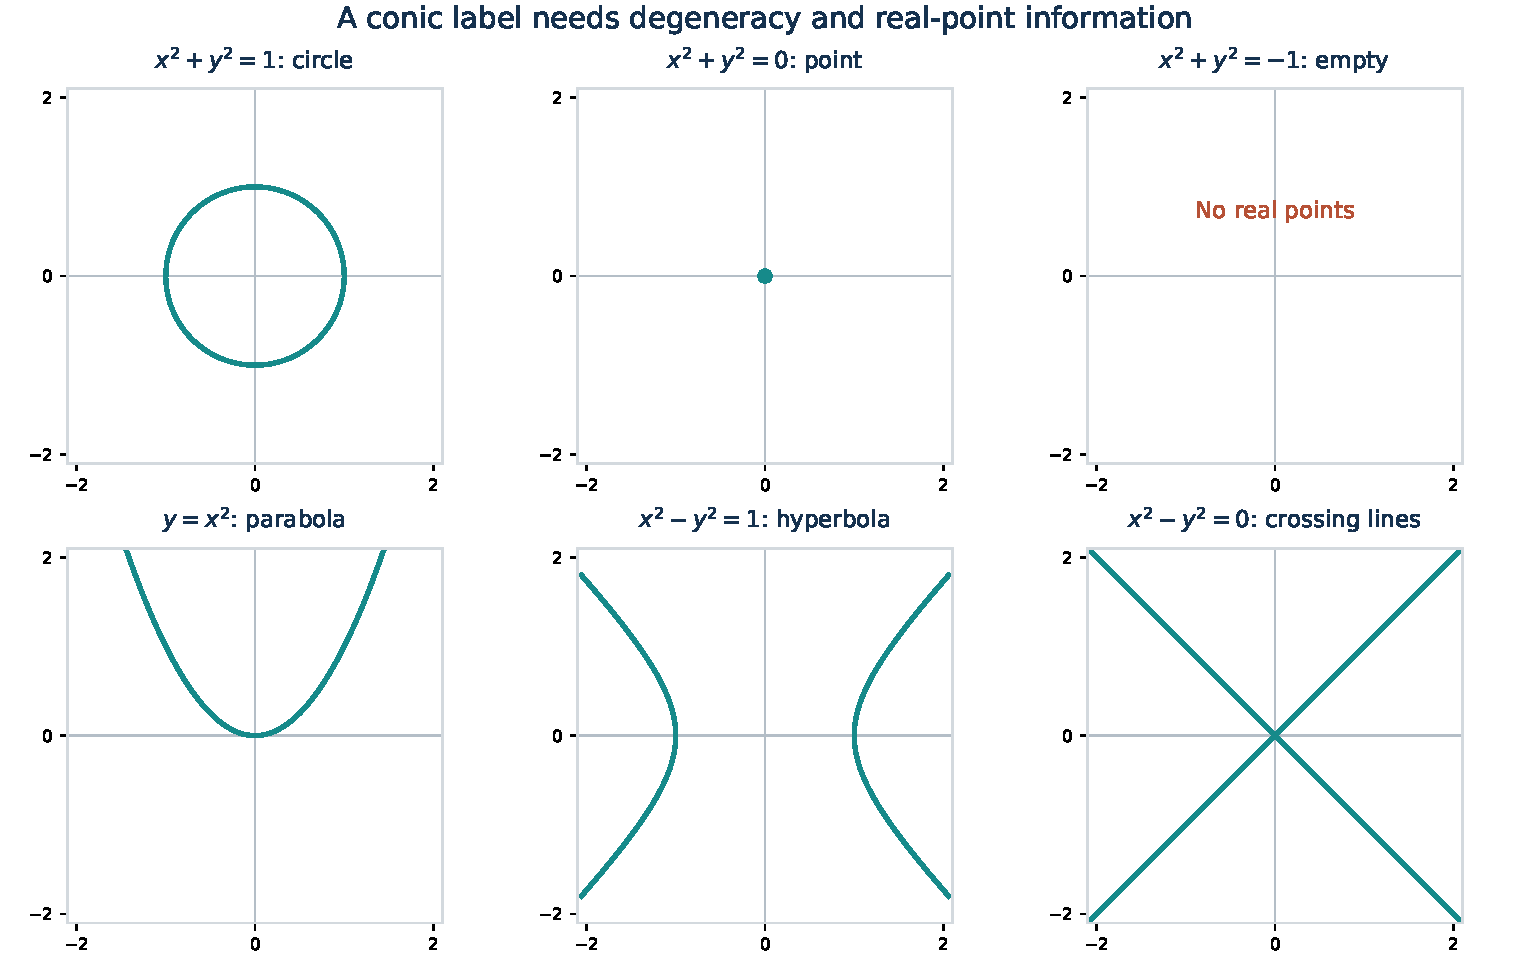
\includegraphics[width=.94\linewidth]{figures/conic_loci.pdf}
\caption{Real loci of explicit rational quadratics. The first row has the
same discriminant $-4$ throughout; the constant term distinguishes a circle,
a point, and an empty locus. The proof of classification uses exact rational
tests, not the plots.}
\end{figure}

Put
\[
 q(x,y)=Ax^2+Bxy+Cy^2+Dx+Ey+F,\qquad
 S=\begin{pmatrix}A&B/2\\B/2&C\end{pmatrix},\quad
 \ell=\binom D E,
\]
and put
\[
 H=\begin{pmatrix}A&B/2&D/2\\B/2&C&E/2\\D/2&E/2&F\end{pmatrix}.
\]
Thus, with $X=(x,y)^T$ and $Z=(x,y,z)^T$,
$q(X)=X^TSX+\ell^TX+F$ and
$q_h(Z)=Z^THZ$ is its homogenization. Homogeneous coordinates mean nonzero
triples modulo multiplication by a nonzero scalar; only this explicitly
described equivalence relation is needed here.

\begin{proposition}[Scaling and coordinate covariance]\label{con:covariance}
Multiplication of all coefficients by a nonzero rational scalar preserves
the zero locus. Under an invertible rational affine substitution $X=MU+t$,
the new quadratic matrix is $M^TSM$. The homogeneous matrix is $T^THT$, where
$T=\left(\begin{smallmatrix}M&t\\0&1\end{smallmatrix}\right)$.
In particular, the substitution and its explicitly computed inverse give
mutually inverse maps of the two zero loci.
\end{proposition}
\begin{proof}
For a nonzero scalar $s$, $sq(X)=0$ implies $q(X)=0$ by multiplication by
$1/s$, and the converse is immediate. Expanding the substitution gives
\[
 q(MU+t)=U^TM^TSMU+(2t^TSM+\ell^TM)U+q(t).
\]
This proves the affine formula, while $(TZ)^TH(TZ)=Z^T(T^THT)Z$ proves
the homogeneous formula. The inverse is $U=M^{-1}(X-t)$, with
$M^{-1}=\operatorname{adj}(M)/\det M$. These are rational operations on a
fixed number of coordinates, with the guard $\det M\ne0$ checked before
division.
\end{proof}

\begin{theorem}[Discriminant and projective singularity]\label{con:invariants}
Let $\Delta=B^2-4AC$. Under the preceding affine substitution,
$\Delta'=(\det M)^2\Delta$. A projective conic is singular, in the sense
that some nonzero homogeneous vector $Z$ satisfies $HZ=0$, if and only if
$\det H=0$. For rational coefficients, existence of such a singular vector
is decided and witnessed by finite rational elimination. When $\det H\ne0$,
no entire affine line is contained in the conic.
\end{theorem}
\begin{proof}
The equality $\Delta=-4\det S$ and determinant multiplication give the
first formula. If $HZ=0$ and $Z\ne0$, an inverse for $H$ would force $Z=0$;
thus $\det H\ne0$ is impossible. Conversely, if the determinant vanishes,
ordinary elimination in three columns chooses the first nonzero rational
pivot when one exists. At least one column is free. Set its free variable
to $1$, the other free variables to $0$, and back-substitute. This produces
a nonzero rational null vector. It also satisfies $q_h(Z)=Z^THZ=0$;
the homogeneous partial derivatives are the coordinates of $2HZ$.

For the last assertion, use an invertible rational affine change sending
a proposed rational affine line to $v=0$. Vanishing identically on it
forces the constant, $u$, and $u^2$ coefficients to vanish. The transformed
polynomial is therefore $v(\alpha u+\beta v+\gamma)$. Its homogeneous
matrix is a sum of two matrices of rank at most one, so has determinant
zero, a fact also obtained by expanding its $3$ by $3$ determinant.
For a line given by represented-real data with certified invertible
coordinate change the same identity applies. Thus a nonsingular conic
cannot contain such a line.
\end{proof}

\begin{lemma}[Rational completion of squares]\label{con:completion}
If $A\ne0$, set
\[
 u=x+\frac{B}{2A}y+\frac{D}{2A},\quad
 K=C-\frac{B^2}{4A},\quad
 L=E-\frac{BD}{2A},\quad M_0=F-\frac{D^2}{4A}.
\]
Then $q=Au^2+Ky^2+Ly+M_0$. If also $K\ne0$, setting
$v=y+L/(2K)$ and $J=M_0-L^2/(4K)$ gives $q=Au^2+Kv^2+J$.
Every nonzero binary quadratic part can be brought to the case $A\ne0$
by an explicitly invertible rational linear change.
\end{lemma}
\begin{proof}
Expanding $Au^2$ gives the original $Ax^2+Bxy+Dx$ and adds
$B^2y^2/(4A)+BDy/(2A)+D^2/(4A)$. The displayed values of $K,L,M_0$
subtract exactly those three additions. The second completion follows
by expanding $K(y+L/(2K))^2$.
If $A=0$ and $C\ne0$, exchange $x$ and $y$. If $A=C=0$ but $B\ne0$,
put $x=r+s$, $y=r-s$; then $Bxy=B r^2-Bs^2$ and the change has
determinant $-2$. These exhaust the nonzero cases by decidable rational
tests. The displayed transformations have explicit rational inverses.
\end{proof}

\begin{theorem}[Exhaustive real-locus classification for rational conics]
\label{con:classification}
There is a primitive recursive procedure returning an invertible rational
affine change and one of the following descriptions. Subsequent positive
rescalings by represented square roots identify the named standard shapes.
For crossing components, the constructive output is their factored
equation; membership in a chosen component for arbitrary represented-real
points is asserted only with a branch certificate or separation from the
crossing. The ordinary shape names in the table carry this qualification.
\begin{center}
\begin{tabular}{p{.27\linewidth}p{.64\linewidth}}
Normal equation and guard & Real zero locus\\\hline
$Au^2+Kv^2=-J$, $AK>0$ & An ellipse if $-J/A>0$; one point if $J=0$;
empty if $-J/A<0$.\\
$Au^2+Kv^2=-J$, $AK<0$ & A hyperbola if $J\ne0$; two intersecting lines
if $J=0$.\\
$Au^2+Ly+M_0=0$, $L\ne0$ & A parabola.\\
$Au^2+M_0=0$ & Two parallel lines if $-M_0/A>0$; one repeated line if
$M_0=0$; empty if $-M_0/A<0$.\\
$Dx+Ey+F=0$ & A line if $(D,E)\ne(0,0)$; the whole plane if $D=E=F=0$;
empty otherwise.
\end{tabular}
\end{center}
Here $A\ne0$ in the first four rows. In the nondegenerate, nonempty cases,
$\Delta<0$, $\Delta=0$, and $\Delta>0$ distinguish ellipse, parabola, and
hyperbola respectively. The negative-discriminant test alone does not
assert nonemptiness.
\end{theorem}
\begin{proof}
Apply Lemma~\ref{con:completion}. If $K\ne0$ the equation is diagonal.
When $A,K$ have the same sign, divide by $A$; the left side is a sum
of two nonnegative squares with positive coefficients. A negative right
side is impossible, a zero right side forces both coordinates to vanish,
and a positive right side gives a rescaled unit circle. More explicitly,
if $R=-J/A>0$, write $u=\sqrt R\,U$ and
$v=\sqrt{R A/K}\,V$ to obtain $U^2+V^2=1$.

When $AK<0$ and $J\ne0$, multiply the equation by the sign of $-J$,
divide by $|J|$, and rescale the two coordinates by positive square roots.
One obtains $U^2-V^2=1$, after exchanging coordinates if necessary.
If $J=0$, the identity
$u^2-(-K/A)v^2=(u-\sqrt{-K/A}\,v)(u+\sqrt{-K/A}\,v)$
gives the two lines. The union statement has a constructive meaning:
for an arbitrary represented-real point one has the product identity,
and membership in a particular line needs a supplied branch, or positive
separation from their intersection. There is no unguarded decision of
which line contains a point at their crossing.

When $K=0$ but $L\ne0$, solve
$y=-Au^2/L-M_0/L$, an invertible affine image of a parabola. If $K=L=0$,
the equation reduces to $u^2=-M_0/A$ and gives the stated alternatives.
For a positive right side the roots have a positive separation, so their
branches can be chosen from a sufficiently accurate rational observation.
The linear case is solved by choosing a nonzero coefficient.

All branches here test rational data and the number of elimination steps
is fixed. In the diagonal rank-two case, $\Delta=-4AK$ up to a positive
square factor; in rank one it is zero. The parabola row has $L\ne0$.
This proves the final classification with the necessary degeneracy and
nonemptiness qualifications. In particular, $x^2+y^2+1=0$ is an explicit
empty negative-discriminant example.
\end{proof}

\begin{theorem}[Constructive principal axes, circles, and rectangular hyperbolas]
\label{con:axes}
For a rational symmetric matrix $S$, an orthonormal eigenbasis can be
constructed by rational operations and nonnegative square roots. Its
eigenvalues are
\[
 \lambda_\pm=\frac{A+C\pm\sqrt{(A-C)^2+B^2}}2.
\]
For a nonempty nondegenerate ellipse, the curve is a circle precisely
when $A=C$ and $B=0$. For a nondegenerate hyperbola its two asymptotic
directions are perpendicular precisely when $A+C=0$.
\end{theorem}
\begin{proof}
If $B=0$, the coordinate axes already form an eigenbasis. If $B\ne0$,
take $v=(B,2(\lambda_+-A))$. The characteristic equation
$(\lambda-A)(\lambda-C)-B^2/4=0$ verifies $Sv=\lambda_+v$.
The vector $v$ is nonzero with $\|v\|\ge |B|$; thus normalization has
a rational lower bound on its denominator. Its perpendicular
$w=(-v_2,v_1)$ has eigenvalue $\lambda_-$, because symmetry makes $Sw$
orthogonal to $v$ and its coefficient is the trace minus $\lambda_+$.
Normalizing $v,w$ gives the promised rotation. Translation to the center
then gives the usual principal-axis equation when $\det S\ne0$.

The two ellipse semiaxes are equal exactly when the two eigenvalues are
equal. Their squared difference is $(A-C)^2+B^2$, which vanishes exactly
when $A=C$ and $B=0$. For a hyperbola, after multiplying the equation
by $-1$ if needed, the diagonal quadratic part has coefficients
$\alpha>0$ and $-\beta<0$. Its asymptotic directions can be taken as
$(\sqrt\beta,\sqrt\alpha)$ and $(\sqrt\beta,-\sqrt\alpha)$.
Their dot product is $\beta-\alpha$, zero exactly when the trace
$\alpha-\beta$ vanishes. Orthogonal changes preserve dot products and
the original trace is $A+C$.
\end{proof}

\subsection{Intersections and rational parametrizations}

\begin{theorem}[Complete quadratic solver with degeneracies]\label{con:roots}
For rational $a,b,c$, the real solutions of $at^2+bt+c=0$ are determined
by a primitive recursive case distinction. If $a\ne0$, put
$\delta=b^2-4ac$. There are no roots for $\delta<0$, the single root
$-b/(2a)$ for $\delta=0$, and the two distinct represented roots
\[
 t_\pm=\frac{-b\pm\sqrt\delta}{2a}
\]
for $\delta>0$. In the latter case
$t_++t_-=-b/a$ and $t_+t_-=c/a$.
If $a=0\ne b$ the only root is $-c/b$. If $a=b=0$, there are all
parameters or none according as $c=0$ or $c\ne0$.
\end{theorem}
\begin{proof}
For $a\ne0$, direct expansion yields
\[
 4a(at^2+bt+c)=(2at+b)^2-\delta.
\]
A square cannot be negative; a zero square has zero base. For $\delta>0$,
let $r=\sqrt\delta$. The two displayed values satisfy the equation,
and their difference is $r/a\ne0$. Conversely, a root has
$(2at+b)^2=r^2$. Put $h=\min(1,\delta)$, so $r\ge h>0$, and obtain
a rational approximation $s_0$ to $s=2at+b$ with error at most $h/4$.
If $s_0\ge0$, then $s+r\ge3h/4$; cancel that guarded factor in
$(s-r)(s+r)=0$ to obtain $s=r$. If $s_0<0$, then $r-s\ge3h/4$;
cancel it instead to obtain $s=-r$. Thus this completeness assertion
uses positive separation and one rational test, not real trichotomy.
Adding and multiplying the formulas
proves the two Vieta identities. The remaining cases are linear
identities with rational zero tests.
\end{proof}

\begin{corollary}[Line--conic intersection]\label{con:line-intersection}
For a rational conic and a rational line $P+tv$ with $v\ne0$, intersections
are obtained by the preceding solver with
\[
 \alpha=v^TSv,\qquad \beta=2P^TSv+\ell^Tv,\qquad \gamma=q(P).
\]
A line is contained in the conic exactly when $\alpha=\beta=\gamma=0$.
Otherwise it has at most two distinct intersections, and the solver
constructs all of them, including tangent and linear cases.
\end{corollary}
\begin{proof}
Expanding $q(P+tv)$ gives $\alpha t^2+\beta t+\gamma$.
If it vanishes identically, evaluation at $0,1,-1$ gives
$\gamma=0$, $\alpha+\beta=0$, and $\alpha-\beta=0$, hence all three
coefficients vanish. The converse is immediate. A nonzero component
of $v$ makes the parametrization injective, so distinct intersection
points correspond to distinct roots. Theorem~\ref{con:roots} supplies
the stated exhaustive list.
\end{proof}

\begin{theorem}[Parametrization from one rational point]\label{con:rational-point}
Let a rational conic have $\det H\ne0$ and a specified rational point $P$.
For each rational direction $v\ne0$ with $\alpha=v^TSv\ne0$, the point
\[
 R(v)=P-\frac{2P^TSv+\ell^Tv}{v^TSv}\,v
\]
lies on the conic. Every rational point $Q\ne P$ is obtained in this way
by taking $v=Q-P$. Two slope charts $v=(1,t)$ and $v=(0,1)$ suffice.
No assertion that an arbitrary rational conic has a rational point is
being made.
\end{theorem}
\begin{proof}
Since $q(P)=0$, the restriction to the line is
$t(\alpha t+\beta)$, where $\beta=2P^TSv+\ell^Tv$.
Its second root is $-\beta/\alpha$, proving the formula.
For $v=Q-P$, substitution at $t=1$ gives $\alpha+\beta=0$.
If $\alpha=0$, then $\beta=0$ and the entire line is contained in the
conic, contrary to Theorem~\ref{con:invariants}. Thus $R(v)=P+v=Q$.
Any rational nonzero direction has either first coordinate nonzero,
in which case it is a scalar multiple of $(1,t)$, or is vertical.
The formula is unchanged by rescaling $v$. This is a finite rational
chart selection. For represented-real points the same recovery is
valid on a specified chart with certified nonzero denominator.
\end{proof}

\begin{proposition}[Standard rational parametrizations]\label{con:standard-param}
For positive rational $a,b,p$, the following rational maps take their
parameters into the indicated curves:
\[
 \begin{array}{ll}
 x=a\dfrac{1-t^2}{1+t^2},\quad y=b\dfrac{2t}{1+t^2}
   & x^2/a^2+y^2/b^2=1,\\[6pt]
 x=a\dfrac{1+t^2}{1-t^2},\quad y=b\dfrac{2t}{1-t^2},\quad t^2\ne1
   & x^2/a^2-y^2/b^2=1,\\[6pt]
 x=pt^2,\quad y=2pt & y^2=4px.
 \end{array}
\]
The first two maps cover all rational points except $(-a,0)$, with
inverse $t=ay/[b(a+x)]$. The last covers every rational point and has
inverse $t=y/(2p)$. Setting $a=b=1$ gives the rational unit circle.
\end{proposition}
\begin{proof}
The identities $(1-t^2)^2+4t^2=(1+t^2)^2$ and
$(1+t^2)^2-4t^2=(1-t^2)^2$ prove the first two assertions; the last
is immediate by squaring. At a point on either of the first two curves,
$x=-a$ forces $y=0$. Otherwise substitute the stated inverse and use
$y^2/b^2=1-x^2/a^2$ or $y^2/b^2=x^2/a^2-1$, respectively.
For the hyperbola this also proves $1-t^2\ne0$, since its simplification
is $2a/(a+x)$. The parabola inverse gives $pt^2=y^2/(4p)=x$.
All denominators are either at least $1$ or explicitly guarded.
\end{proof}

\subsection{Foci, directrices, and optical laws}

\begin{theorem}[Ellipse: focal and Cartesian definitions agree]\label{con:ellipse-foci}
Let $a\ge b>0$, let $c\ge0$ satisfy $c^2=a^2-b^2$, and let
$d_-=\sqrt{(x+c)^2+y^2}$, $d_+=\sqrt{(x-c)^2+y^2}$.
Then
\[
 x^2/a^2+y^2/b^2=1\quad\Longleftrightarrow\quad d_-+d_+=2a.
\]
On the ellipse, $d_-=a+cx/a$ and $d_+=a-cx/a$.
Here the parameters may be rational or fixed represented-real parameters
with the displayed positive bounds; rational $a,b$ supply such bounds
automatically for the constructed $c$.
\end{theorem}
\begin{proof}
The Cartesian equation gives $|x|\le a$ and
$y^2=b^2(1-x^2/a^2)$. Therefore
\[
 (x\pm c)^2+y^2=(a\pm cx/a)^2.
\]
Both quantities $a\pm cx/a$ are nonnegative, indeed at least
$a-c=b^2/(a+c)>0$. Uniqueness of nonnegative square roots proves the
two distance formulas and hence their sum. Conversely,
$d_-^2-d_+^2=4cx$. Factoring this as
$(d_--d_+)(d_-+d_+)$ and using the given sum yields
$d_--d_+=2cx/a$. Adding and subtracting give the same distance
formulas. Squaring $d_+=a-cx/a$ and canceling $-2cx$ gives
\[
 (1-c^2/a^2)x^2+y^2=a^2-c^2=b^2.
\]
Since $1-c^2/a^2=b^2/a^2$ and $b>0$, this is the Cartesian equation.
Every squaring step in the forward direction retained the required sign.
\end{proof}

\begin{theorem}[Hyperbola: focal and Cartesian definitions agree]\label{con:hyperbola-foci}
Let $a,b>0$, $c\ge0$, and $c^2=a^2+b^2$, and define $d_-,d_+$ as above.
Then
\[
 x^2/a^2-y^2/b^2=1\quad\Longleftrightarrow\quad |d_--d_+|=2a.
\]
On the branch $x\ge a$, $d_-=cx/a+a$ and $d_+=cx/a-a$.
The other branch follows by replacing $x$ by $-x$.
\end{theorem}
\begin{proof}
The Cartesian equation implies $x^2\ge a^2$. Approximate $x$ by rational
$x_0$ to error at most $a/4$. If $x_0\ge0$, then $x+a\ge3a/4$;
division of $(x-a)(x+a)=x^2-a^2\ge0$ by this positive factor gives
$x\ge a$. If $x_0<0$, use $a-x\ge3a/4$ in the reflected argument
to obtain $x\le-a$. On the right branch, substituting
$y^2=b^2(x^2/a^2-1)$ gives
\[
 (x+c)^2+y^2=(cx/a+a)^2,\qquad
 (x-c)^2+y^2=(cx/a-a)^2.
\]
The second base is at least $c-a=b^2/(c+a)>0$; hence the displayed
distance formulas are valid and their difference is $2a$. Reflection
in the $y$ axis interchanges the distances.

Conversely, positive separation of $d_--d_+$ chooses one of its two
signs. Suppose first $d_--d_+=2a$. Difference of squares now gives
$d_-+d_+=2cx/a$, hence $d_+=cx/a-a$. Squaring and canceling gives
\[
 (c^2/a^2-1)x^2-y^2=c^2-a^2=b^2,
\]
which is precisely the desired equation. The other sign is its reflected
copy. The branch selections have an explicit positive gap $a$ or $2a$;
they are not appeals to unrestricted real excluded middle.
\end{proof}

\begin{theorem}[Parabola: focus and directrix]\label{con:parabola-foci}
For $p>0$, a point has equal distance from the focus $(p,0)$ and the
directrix $x=-p$ exactly when $y^2=4px$.
\end{theorem}
\begin{proof}
The two squared distances are $(x-p)^2+y^2$ and $(x+p)^2$.
Equality is therefore equivalent to $y^2=4px$. Equality of their
nonnegative square roots is equivalent to equality of their squares.
If the equation holds then $x\ge0$, and the common distance is $x+p$;
this positive formula will also be used in the reflection law below.
\end{proof}

\begin{theorem}[Eccentricity and a guarded polar equation]\label{con:directrix}
For rational $d,e>0$, the distance-ratio locus with focus $(0,0)$,
directrix $x=d$, and eccentricity $e$ is
\[
 (1-e^2)x^2+y^2+2e^2dx-e^2d^2=0.
\]
It is a nonempty nondegenerate ellipse, parabola, or hyperbola according
as $e<1$, $e=1$, or $e>1$. On a unit-direction chart $(c,s)$ with
$c^2+s^2=1$ and $1+ec>0$, the part on the side $x\le d$ is
\[
 (x,y)=r(c,s),\qquad r=\frac{ed}{1+ec}.
\]
The equation describes exactly those points of this ray satisfying the
distance-ratio condition on that side.
\end{theorem}
\begin{proof}
The distance-ratio condition is
$\sqrt{x^2+y^2}=e|x-d|$. Squaring gives the displayed equation and
nonnegativity makes the converse valid. Its discriminant is
$-4(1-e^2)$ and its homogeneous determinant is $-e^2d^2\ne0$.
The rational point $(ed/(1+e),0)$ belongs to it, so it is nonempty;
Theorem~\ref{con:classification} now gives its type.
On the indicated side, $r=e(d-rc)$, hence $r(1+ec)=ed$.
Conversely the formula has $r>0$ and
$d-rc=d/(1+ec)>0$, which proves both the side condition and the
distance identity. On the opposite side a separate guarded formula
$r=ed/(ec-1)$ applies when $ec-1>0$. Thus a hyperbola's second side
is not silently discarded by removing an absolute value.
\end{proof}

\begin{theorem}[Quadratic tangents and second-order contact]\label{con:tangent}
If $q(P)=0$, write $g=2SP+\ell$. For every displacement $h$,
\[
 q(P+h)=g^Th+h^TSh.
\]
If $g$ is nonzero (with an apartness bound for represented data), the
tangent line is $g^Th=0$. For a tangent direction $v$,
$q(P+tv)=t^2v^TSv$; if $v^TSv\ne0$, the intersection has exactly the
double parameter root $t=0$. For a nonsingular projective conic this
last coefficient cannot vanish. The standard tangent equations are
\[
 \frac{x_0x}{a^2}+\frac{y_0y}{b^2}=1,\quad
 \frac{x_0x}{a^2}-\frac{y_0y}{b^2}=1,\quad
 y_0y=2p(x+x_0)
\]
for ellipse, hyperbola, and parabola at $(x_0,y_0)$, respectively.
\end{theorem}
\begin{proof}
Expand $(P+h)^TS(P+h)$; symmetry of $S$ makes the mixed terms
$2P^TSh$. The constant is $q(P)=0$, giving the identity.
Its linear part is zero precisely on the displayed line, and substituting
$h=tv$ gives the contact statement. If the quadratic coefficient also
vanished, the entire line would be contained in the conic, contradicting
Theorem~\ref{con:invariants}. In a nonsingular projective conic, $g=0$
at an affine point is impossible: Euler's identity for $q_h$ would
also force its third partial derivative to vanish, giving $H(P,1)^T=0$.
Finally substitute the three standard equations into $g^T(X-P)=0$,
and simplify using the equation satisfied by $P$.
This exact expansion is also a quantitative differentiability proof:
on $\|h\|_\infty\le1$ the remainder is bounded by
$(|A|+|B|+|C|)\|h\|_\infty^2$.
\end{proof}

\begin{proposition}[Polar reciprocity and poles]\label{con:polar}
For a homogeneous conic with symmetric matrix $H$, define the polar of
a nonzero vector $P$ by $P^THX=0$. Then $Q$ lies on the polar of $P$
if and only if $P$ lies on the polar of $Q$. If $\det H\ne0$, every
projective line $L^TX=0$ has the unique projective pole $H^{-1}L$.
At a regular point of the conic, meaning $HP\ne0$ with an apartness
certificate when needed, its polar is its tangent. Every point is regular
when $\det H\ne0$.
\end{proposition}
\begin{proof}
Symmetry gives $P^THQ=Q^THP$, which proves reciprocity.
When $H$ is invertible, $H^{-1}L$ is nonzero and
$(H^{-1}L)^THX=L^TX$. Conversely equality of projective line
coefficients up to a nonzero scalar gives the same equality of pole
vectors after multiplication by $H^{-1}$. At a regular conic point the
homogeneous linearization is $2P^THX=0$, a genuine line because its
coefficient vector is nonzero, so it is exactly the polar.
Inverses and equality tests for rational input use guarded rational
matrix operations.
\end{proof}

\begin{theorem}[Ellipse reflection law]\label{con:ellipse-reflection}
At a point $P$ of the ellipse in Theorem~\ref{con:ellipse-foci}, reflection
in the tangent sends the incoming unit direction from one focus to the
outgoing unit direction towards the other focus.
\end{theorem}
\begin{proof}
Let $u=(P-(-c,0))/d_-$ and $v=(P-(c,0))/d_+$. Both are unit vectors.
The focal formulas, whose denominators are positive, give
\[
 u+v=\frac{2ab^2}{d_-d_+}\,(x/a^2,y/b^2).
\]
For example, the first coordinate numerator is
$(x+c)(a-cx/a)+(x-c)(a+cx/a)=2b^2x/a$;
the second is $2ay$. Thus $u+v$ is a nonzero normal to the tangent.
It is quantitatively nonzero: the ellipse equation gives
$x^2/a^4+y^2/b^4\ge1/a^2$, and $d_-d_+\le a^2$, so
$\|u+v\|^2\ge4b^4/a^4>0$. Reflection in a line with normal $n$ sends $w$ to
$w-2(w\cdot n)n/(n\cdot n)$. With $n=u+v$,
\[
 2u\cdot n=2(1+u\cdot v)=n\cdot n.
\]
Consequently the reflected direction is $u-(u+v)=-v$, precisely the
unit direction from $P$ towards the second focus. This proves the
optical law as a vector identity without choosing angle branches.
\end{proof}

\begin{theorem}[Parabola reflection law]\label{con:parabola-reflection}
For $p>0$, reflection in the tangent to $y^2=4px$ sends the incoming
direction $(-1,0)$ to the unit direction from the point of incidence
towards the focus $(p,0)$.
\end{theorem}
\begin{proof}
At $P=(x,y)$ put $u=(x-p,y)/(x+p)$ and $e=(-1,0)$.
The common-distance formula in Theorem~\ref{con:parabola-foci} gives
$\|u\|=1$, and $x+p>0$. Moreover
\[
 u+e=\frac{(-2p,y)}{x+p}
\]
is a nonzero normal to the parabola. A rational upper bound $M$ for
$x+p$ gives $\|u+e\|^2\ge4p^2/M^2>0$, explicitly guarding the
reflection denominator. Since $u,e$ are unit vectors,
$2e\cdot(u+e)=\|u+e\|^2$. The same reflection formula gives
$e-(u+e)=-u$, which points from $P$ to the focus.
\end{proof}

\begin{proposition}[Hyperbola asymptotes with a modulus]\label{con:asymptotes}
On the upper right branch of $x^2/a^2-y^2/b^2=1$, $a,b>0$,
\[
 0\le \frac ba x-y
 =\frac{ab}{x+\sqrt{x^2-a^2}}\le\frac{ab}{x}\qquad(x\ge a).
\]
Thus $x\ge\max(a,ab\,2^n)$ makes the vertical deviation from
$y=(b/a)x$ at most $2^{-n}$. The other asymptotes follow by coordinate
reflections. The change $u=x/a+y/b$, $v=x/a-y/b$ gives $uv=1$.
\end{proposition}
\begin{proof}
The branch equation gives $y=(b/a)\sqrt{x^2-a^2}$.
Multiply $x-\sqrt{x^2-a^2}$ by its conjugate; the numerator is $a^2$.
The denominator is at least $x>0$, giving the displayed inequality
and its explicit cutoff. The formula $uv=x^2/a^2-y^2/b^2$ proves
the last assertion. No qualitative limit or unbounded search is used.
\end{proof}

\begin{theorem}[Parallel chord midpoints and conjugate diameters]
\label{con:diameters}
For the centered conic $X^TSX=1$, a chord in direction $v$ with
$v^TSv\ne0$ has midpoint
\[
 M=P-\frac{P^TSv}{v^TSv}\,v,
 \qquad M^TSv=0.
\]
Hence the midpoints of parallel chords lie on the diameter $X^TSv=0$.
Conjugacy of directions, $u^TSv=0$, is symmetric. For an ellipse,
the conjugate semidiameter vectors
$u=(ac,bs)$, $v=(-as,bc)$ with $c^2+s^2=1$ satisfy
\[
 \|u\|^2+\|v\|^2=a^2+b^2,\qquad \det(u,v)=ab.
\]
\end{theorem}
\begin{proof}
On $P+tv$ the quadratic coefficient is $v^TSv$ and the linear
coefficient is $2P^TSv$. Vieta's root-sum formula makes the average
parameter $-P^TSv/(v^TSv)$, proving the midpoint expression.
Multiplying it by $Sv$ gives zero. Symmetry of $S$ proves reciprocity
of the two directions. For the final identities, expand the four
squared coordinates and collect the factors $c^2+s^2$; the sum is
$(a^2+b^2)(c^2+s^2)$ and the determinant is $ab(c^2+s^2)$.
For $S=\operatorname{diag}(a^{-2},b^{-2})$, the two vectors are on
the ellipse and $u^TSv=-cs+sc=0$, justifying their description.
\end{proof}

\section{Quadrics in three dimensions}
\label{sec:quadrics}

Here a quadric is the zero locus of $q(X)=X^TQX+\ell^TX+f$,
where $Q$ is a rational symmetric $3$ by $3$ matrix. A nonsymmetric
input matrix may first be replaced by $(Q+Q^T)/2$, because the skew
part contributes zero to $X^TQX$.

\begin{theorem}[Finite rational reduction of every quadric]\label{con:quadric-reduction}
An explicitly bounded rational elimination algorithm takes every such
polynomial to one of the forms
\[
 \lambda_1u_1^2+\cdots+\lambda_ru_r^2=K,
 \qquad
 \lambda_1u_1^2+\cdots+\lambda_ru_r^2+w=0,
\]
by an invertible rational affine change, with $0\le r\le3$ and all
$\lambda_i\ne0$. The second form has $r\le2$ and $w$ is one of the
remaining independent coordinates. Zero-dimensional sums are allowed.
The algorithm and correctness proof use at most three quadratic pivots.
\end{theorem}
\begin{proof}
If some diagonal entry is nonzero, choose it as pivot. Completing its
square removes every mixed term involving that variable and leaves
a symmetric quadratic form on one fewer variable. If every diagonal
entry is zero but $q_{ij}\ne0$, replace the basis vector $e_i$ by
$e_i+e_j$, leaving the others fixed. The new diagonal entry is
$2q_{ij}\ne0$ and the basis change has determinant $1$. Thus a pivot
is available whenever the quadratic form is nonzero. Repeat at most
three times to obtain $\sum_i\lambda_i u_i^2$ plus a linear form.

For each nonzero $\lambda_i$, translate $u_i$ by its linear coefficient
divided by $2\lambda_i$. This removes the linear terms in these
coordinates. Only a linear form on the null coordinates remains.
If it vanishes, move the constant to the right and obtain the first
form. Otherwise choose a nonzero rational coefficient of that residual
linear form and replace its coordinate by the entire linear form plus
the constant. This invertible change gives the second form. All searches
range over at most three coordinates, every pivot test is rational,
and every division has its selected nonzero pivot as guard. This is
a direct fixed-length correctness argument, not a use of an unrestricted
spectral theorem.
\end{proof}

\begin{corollary}[Exhaustive affine types of rational quadrics]\label{con:quadric-types}
The preceding reduction decides the real affine type, with represented
positive rescalings, as follows. As in Theorem~\ref{con:classification},
an intersecting-plane output is its factored equation; it does not decide
which component contains an arbitrary represented-real point at their
crossing. A nonzero residual linear term gives
an elliptic paraboloid for $r=2$ with equal quadratic signs, a hyperbolic
paraboloid for $r=2$ with opposite signs, a parabolic cylinder for $r=1$,
and a plane for $r=0$. Without that term:
\begin{itemize}
\item Rank three definite forms give an ellipsoid, a point, or the empty
set according to the sign of $K$ relative to the quadratic coefficients.
Rank three indefinite forms with $K=0$ give a cone; for $K\ne0$ they
give a one-sheet or two-sheet hyperboloid according as, after making
the right side positive, there are two or one positive coefficients.
\item Rank two forms give a cylinder over the corresponding planar
diagonal conic: elliptic or hyperbolic cylinders, a line, intersecting
planes, or the empty set, with the signs specified in
Theorem~\ref{con:classification}.
\item Rank one gives two parallel planes, one repeated plane, or the
empty set. Rank zero gives all space or the empty set.
\end{itemize}
\end{corollary}
\begin{proof}
Substitute $u_i=U_i/\sqrt{|\lambda_i|}$ for each nonzero quadratic
coefficient; when $K\ne0$, also scale using
$\sqrt{|K|}$. Thus only signs and whether $K$ is zero remain.
For definite forms a sum of squares is nonnegative and is zero only
when all terms vanish. For indefinite rank-three forms the resulting
equations are $u^2+v^2-w^2=1$, $u^2-v^2-w^2=1$, or a homogeneous
cone equation, after renaming coordinates and possibly multiplying
by $-1$. These equations are the definitions of the named affine
types. A null coordinate is free, so rank two is exactly the product
of its planar locus with a line; rank one is the product of its
one-variable locus with a plane. For a residual linear coordinate,
solve for $w$ and inspect the one or two quadratic signs. The list
is exhaustive because the reduction has no other output forms.
The names classify these explicit equations; no additional claim
about a global topological decision procedure is required.
\end{proof}

\begin{theorem}[Stereographic rational parametrization of the sphere]
\label{con:sphere-param}
The map
\[
 (u,v)\longmapsto
 \left(\frac{2u}{1+u^2+v^2},
       \frac{2v}{1+u^2+v^2},
       \frac{u^2+v^2-1}{1+u^2+v^2}\right)
\]
parametrizes the unit sphere except its north pole $(0,0,1)$.
Its inverse is $(u,v)=(x/(1-z),y/(1-z))$. In particular it gives
all rational points except the pole by rational parameters.
For represented-real input the inverse is a chart with a supplied
lower bound on $|1-z|$.
\end{theorem}
\begin{proof}
Put $s=u^2+v^2$. The sum of squared numerators is
$4s+(s-1)^2=(s+1)^2$, proving the sphere equation.
Furthermore $1-z=2/(1+s)>0$, so the image omits the north pole and
the stated inverse recovers $u,v$. Conversely, if $x^2+y^2+z^2=1$
and $z\ne1$, then
\[
 u^2+v^2=\frac{x^2+y^2}{(1-z)^2}=\frac{1+z}{1-z}.
\]
Substitution recovers $x,y,z$. The forward denominator is at least
$1$, so the forward map is uniformly total on rational input.
Translations and positive radius scaling give the analogous formula
for any specified sphere.
\end{proof}

\begin{theorem}[Two rulings of a hyperbolic paraboloid and a hyperboloid]
\label{con:rulings}
The surface $z=xy$ is covered by each of the line families
$(t,s,ts)$ and $(s,t,st)$, with $t$ fixed and $s$ variable.
The one-sheet hyperboloid $x^2+y^2-z^2=1$ has the two line families
\[
 (x,y,z)=(c-st,s+ct,\varepsilon t),\qquad
 c^2+s^2=1,\quad\varepsilon\in\{-1,1\}.
\]
Through each of its points there is exactly one line of each displayed
family, and the two lines are distinct. A positive definite ellipsoid
contains no entire nonconstant affine line.
\end{theorem}
\begin{proof}
The first formulas satisfy $z=xy$ directly and fix either the first
or second coordinate. For the hyperboloid,
$(c-st)^2+(s+ct)^2=(c^2+s^2)(1+t^2)=1+t^2$.
Given a point $(x,y,z)$ on it and a sign $\varepsilon$, set
\[
 t=\varepsilon z,\qquad
 c=\frac{x+ty}{1+t^2},\quad s=\frac{y-tx}{1+t^2}.
\]
These satisfy $c^2+s^2=(x^2+y^2)/(1+t^2)=1$ and invert the
displayed parametrization, proving coverage and uniqueness within
each family. The two lines are distinct: if they coincided, their unique
intersections with $z=0$ would give the same base $(c,s)$, but the
directions $(-s,c,1)$ and $(-s,c,-1)$ are not proportional because
$c^2+s^2=1$. Finally restricting a positive definite ellipsoid to
$P+tv$ gives leading coefficient $\sum_i v_i^2/a_i^2$, which can
vanish only when $v=0$. An entire nonconstant line therefore cannot
be contained in it.
\end{proof}

\begin{theorem}[Ellipsoid support plane and unique maximizing point]
\label{con:ellipsoid-support}
For $a_i>0$ and a nonzero normal $n=(n_1,n_2,n_3)$, put
$s=\sqrt{\sum_i a_i^2n_i^2}$. On the ellipsoid
$\sum_i x_i^2/a_i^2=1$,
\[
 n\cdot x\le s,
 \qquad
 p_i=\frac{a_i^2n_i}{s}
\]
is the unique point attaining equality. Thus $n\cdot x=s$ is a
supporting tangent plane. For rational nonzero $n$ and positive
rational $a_i$, a nonzero component supplies a rational lower bound
for $s$, making the construction primitive recursive.
\end{theorem}
\begin{proof}
Write $z_i=x_i/a_i$ and $m_i=a_i n_i$. Then $\sum_i z_i^2=1$ and
$\sum_i m_i^2=s^2$. The finite identity
\[
 \Bigl(\sum_i z_i^2\Bigr)\Bigl(\sum_i m_i^2\Bigr)
 -(\sum_i z_i m_i)^2
 =\sum_{i<j}(z_i m_j-z_j m_i)^2
\]
gives $|n\cdot x|\le s$. The proposed point has $z=m/s$, hence
lies on the ellipsoid and attains $s$. If another point attains it,
\[
 \sum_i(z_i-m_i/s)^2=1+1-2(n\cdot x)/s=0,
\]
so each summand vanishes and the points coincide. The normal to
$\sum_i x_i^2/a_i^2=1$ at $p$ is $(2p_i/a_i^2)_i=2n/s$;
therefore its tangent plane is the displayed supporting plane.
\end{proof}

\paragraph{Arithmetic audit for this chapter.}
The rational classification algorithms have fixed matrix dimension,
bounded coefficient tests, and explicit pivot formulas. Their correctness
reduces to integer polynomial identities and ordered rational inequalities.
Every nonrational output above is built from a finite expression using
guarded division and nonnegative square roots; its precision program is
therefore primitive recursive by the foundations chapter. Reflection laws,
polar reciprocity, and normal-form identities are exact algebraic
identities after clearing certified denominators. Focal and support
statements additionally use nonnegative-square-root uniqueness and finite
sum-of-squares estimates. No algebraically closed field, arbitrary real
root oracle, compactness principle, or unlimited search is needed.

\section{Coordinate systems, trigonometry, and changes of variables}
\label{sec:coordinates}

This chapter addresses the Cartesian, polar, cylindrical and spherical
coordinate links of the source article. Its algebraic direction coordinates
are especially useful constructively: an angle may be represented by its
unit direction $(c,s)$ without choosing a discontinuous global argument.
We also construct the conventional sine and cosine functions with an
explicit finite-series bound, so that the forward radian formulas have
their usual meaning.

\subsection{Radian functions from bounded rational sums}

Identify a pair $(a,b)$ with the formal complex number $a+ib$ only as
notation for the rational multiplication rule
$(a,b)(c,d)=(ac-bd,ad+bc)$. Put
\[
 E_N(t)=\sum_{j=0}^{N}\frac{(it)^j}{j!}=C_N(t)+iS_N(t),
\]
where $C_N$ collects the even powers and $S_N$ the odd powers. These are
finite rational expressions for rational $t$. The norm used for estimates
in this subsection is $|(a,b)|_1=|a|+|b|$, which is submultiplicative by
the rational triangle inequality.

\begin{lemma}[A primitive-recursive trigonometric tail bound]
\label{coord:tail}
Let $M\ge1$ be an integer, $|t|\le M$, and $J\ge N\ge2M$. Then
\[
 |E_J(t)-E_N(t)|_1\le 2^{4M-N}.
\]
Consequently the schedule $N(M,n)=4M+n+6$ defines PR names
$C_{N(M,n)}(t)$ and $S_{N(M,n)}(t)$ for $\cos t$ and $\sin t$.
Different admissible choices of $M$ give equal names.
\end{lemma}
\begin{proof}
For every finite $K$, $j!\ge2^{j-1}$ for $j\ge1$, by induction on $j$.
Hence $\sum_{j=0}^K1/j!\le3$. The multinomial identity, obtained by
repeated distributivity, gives
\[
 \sum_{j=0}^{K}\frac{M^j}{j!}
 \le\left(\sum_{j=0}^{K}\frac1{j!}\right)^M
 \le3^M\le2^{2M}.
\]
The first inequality holds because all terms whose total degree is at
most $K$ occur in the product, with the displayed multinomial coefficients;
the additional terms are nonnegative. Starting at index $2M$, successive
terms $M^j/j!$ decrease by a factor at most $1/2$. Therefore
\[
 \sum_{j=N+1}^{J}\frac{M^j}{j!}
 \le 2^{2M}\sum_{j=N+1}^{J}2^{-(j-2M)}
 \le2^{4M-N}.
\]
All sums here are finite, and the geometric-sum estimate is an induction
identity. The pair triangle inequality proves the assertion for $E$.
The proposed schedule leaves error at most $2^{-n-6}$ after any further
truncation. Comparing two truncations at a common later degree proves
the name condition and independence of $M$. Powers, factorials, finite
sums and the degree schedule are primitive recursive. The multinomial
and geometric-sum proofs use quantifier-free induction on their finite
counters.
\end{proof}

\begin{theorem}[Addition laws and the unit-circle identity]
\label{coord:addition}
The constructed functions satisfy
\begin{align*}
 \cos(s+t)&=\cos s\cos t-\sin s\sin t,\\
 \sin(s+t)&=\sin s\cos t+\cos s\sin t,\\
 \cos^2t+\sin^2t&=1.
\end{align*}
Also $\cos0=1$, $\sin0=0$, $\cos(-t)=\cos t$, and
$\sin(-t)=-\sin t$. The assertions are arithmetic identities of fixed PR
names, first for rational parameters and then for fixed PR named inputs
with supplied magnitude bounds.
\end{theorem}
\begin{proof}
Multiply $E_N(s)E_N(t)$. For total degree $k\le N$, the coefficient is
\[
 i^k\sum_{j=0}^k\frac{s^jt^{k-j}}{j!(k-j)!}
       =i^k\frac{(s+t)^k}{k!}
\]
by the binomial formula. Thus its terms through total degree $N$ equal
$E_N(s+t)$. With an integer $M\ge|s|+|t|+1$, the sum of the absolute
values of the remaining coefficients is bounded by
$\sum_{k=N+1}^{2N}M^k/k!\le2^{4M-N}$.
Lemma~\ref{coord:tail} and the multiplication estimate of
Theorem~\ref{found:operations} give the addition laws at each requested
precision. The parity statements hold term by term in the finite sums.
Set $s=-t$ in the addition formula and use $E_N(0)=(1,0)$ to get the
unit-circle identity. This also proves $|\cos t|,|\sin t|\le1$ from
nonnegativity of squares, through finite rational observations.

To admit named arguments, note that for $|u|,|v|\le M$,
\[
 |E_N(u)-E_N(v)|_1
 \le |u-v|\sum_{j=1}^N\frac{jM^{j-1}}{j!}
 \le3^M|u-v|.
\]
The first inequality is the factorization of $u^j-v^j$; the second is
the finite bound in Lemma~\ref{coord:tail}. Query an argument at precision
$n+\ell(3^{M+1})+8$, allow the approximating value the bound $M+1$,
and use degree $4(M+1)+n+8$. These are PR schedules. The estimates
transfer the rational formulas with room for every observation error.
\end{proof}

\begin{theorem}[Quantitative trigonometric derivatives]
\label{coord:derivatives}
For $|h|\le1$,
\begin{align*}
 |\sin(t+h)-\sin t-h\cos t|&\le6h^2,\\
 |\cos(t+h)-\cos t+h\sin t|&\le6h^2.
\end{align*}
In particular the names have derivatives $\cos t$ and $-\sin t$ in the
finite-error sense, with an explicit modulus.
\end{theorem}
\begin{proof}
The finite series and Lemma~\ref{coord:tail} imply
$|\cos h-1|\le3h^2$ and $|\sin h-h|\le3|h|^3$ for $|h|\le1$:
factor $h^2$ or $|h|^3$ from the corresponding tail and bound the
remaining factorial sum by $3$. For a named $h$ with $|h|\le1$, clip its rational observations to $[-1,1]$ before applying these finite estimates; clipping preserves the name and the error bound. Substitute these estimates into the
addition formulas. Each coefficient $\sin t$ or $\cos t$ has absolute
value at most one. The first residual is
$\sin t(\cos h-1)+\cos t(\sin h-h)$, so it is at most
$3h^2+3|h|^3\le6h^2$; the second is handled by the displayed
cosine addition identity. For a difference quotient error at most
$2^{-n}$ it suffices to supply $0<|h|\le2^{-n}/6$; the quotient is
used only under this nonzero guard. The remainder inequalities themselves
include $h=0$ and avoid division entirely.
\end{proof}

\subsection{Polar and spatial coordinates}

\begin{theorem}[Polar direction coordinates and reconstruction]
\label{coord:polar}
For $r\ge0$ and $c^2+s^2=1$, put $(x,y)=(rc,rs)$. Then
$x^2+y^2=r^2$. Conversely, for a rational point $(x,y)\ne(0,0)$, the
constructed values
\[
 r=\sqrt{x^2+y^2},\qquad c=x/r,\qquad s=y/r
\]
give a unique radius and unit direction and reconstruct the point. At
the origin one may output $r=0,(c,s)=(1,0)$; the direction there is not
unique. For arbitrary fixed PR named points the same converse requires
a supplied positive lower bound on $x^2+y^2$, or the supplied assertion
that both coordinates are zero. The forward radian formulas are
$x=r\cos\theta$, $y=r\sin\theta$.
\end{theorem}
\begin{proof}
The forward assertion is the polynomial identity
$(rc)^2+(rs)^2=r^2(c^2+s^2)$. For a nonzero rational point the positive
rational $q=x^2+y^2$ has a computable rational lower bound. If
$q\ge\delta>0$, then $r\ge\min(1,\delta)$, since
$0<\delta\le1$ implies $\sqrt\delta\ge\delta$, and
$\delta\ge1$ implies $\sqrt\delta\ge1$. A dyadic lower bound below
$\min(1,\delta)$ is found by bounded search. Thus division by $r$ is
permitted by Theorem~\ref{found:operations}. Squaring proves the unit
identity, and multiplying gives reconstruction. Nonnegative-root
uniqueness forces any other nonnegative radius to be $r$, and the
nonzero radius then forces the same direction. The zero case is checked
directly. Theorem~\ref{coord:addition} supplies the forward radian case.
\end{proof}

The usual scalar formula $\theta=\arctan(y/x)$ requires both a chart and
a quadrant convention. No global scalar inverse is claimed here.
Direction coordinates encode the complete ray, including vertical and
negative-horizontal directions. The rational parametrizations of
Theorem~\ref{con:standard-param} give stereographic charts; their inverse
requires the chart denominator to be apart from zero. This is an atlas
interpretation, not a choice of a global continuous argument.

\begin{theorem}[Cylindrical coordinates]
\label{coord:cylindrical}
The transformation
\[
 (r,c,s,z)\longmapsto(rc,rs,z),\qquad r\ge0,\quad c^2+s^2=1,
\]
satisfies $x^2+y^2=r^2$. It has the inverse of
Theorem~\ref{coord:polar} on each horizontal plane, with the same axis
qualification. Hence $x^2+y^2=R^2$ is the circular cylinder of radius
$R\ge0$, and $z=k$ fixes a horizontal plane. Radian input substitutes
$c=\cos\theta,s=\sin\theta$.
\end{theorem}
\begin{proof}
Apply the polar theorem to the first two coordinates and leave $z$
unchanged. The inverse preserves that last coordinate. A fixed radius
condition places no restriction on $z$; fixing $z$ places no restriction
on the first two coordinates. These observations prove the locus
descriptions by the displayed equations. All inverse branches on
rational Cartesian inputs are rational zero tests on $x^2+y^2$.
\end{proof}

\begin{theorem}[Spherical coordinates with explicit axis data]
\label{coord:spherical}
For $\rho\ge0$, $c_\theta^2+s_\theta^2=1$, and
$c_\phi^2+s_\phi^2=1$ with $s_\phi\ge0$, set
\[
 x=\rho s_\phi c_\theta,\quad
 y=\rho s_\phi s_\theta,\quad z=\rho c_\phi.
\]
Then $x^2+y^2+z^2=\rho^2$ and the cylindrical radius is
$r=\rho s_\phi$. For a rational point away from the origin and the
vertical axis an inverse is
\[
 \rho=\sqrt{x^2+y^2+z^2},\quad r=\sqrt{x^2+y^2},\quad
 (c_\theta,s_\theta)=(x/r,y/r),\quad
 (c_\phi,s_\phi)=(z/\rho,r/\rho).
\]
On the nonzero vertical axis take $(c_\theta,s_\theta)=(1,0)$,
$s_\phi=0,c_\phi=\sgn z$. At the origin use $\rho=0$ and arbitrary
fixed admissible directions. The inverse for general named data
requires the corresponding radial gaps or certified axis cases.
\end{theorem}
\begin{proof}
Substitution and the two unit identities give
\[
 x^2+y^2+z^2
 =\rho^2s_\phi^2(c_\theta^2+s_\theta^2)+\rho^2c_\phi^2
 =\rho^2.
\]
The horizontal norm squared is $\rho^2s_\phi^2$; since both factors
are nonnegative, its nonnegative root is $\rho s_\phi$. The inverse
unit identities follow from $r^2=x^2+y^2$ and $\rho^2=r^2+z^2$;
substitution then recovers all three coordinates. The finitely many
axis cases are explicit rational branches. The nonzero denominators
receive gaps exactly as in the polar theorem. For conventional
inclination and azimuth one substitutes
$c_\phi=\cos\phi,s_\phi=\sin\phi$ and
$c_\theta=\cos\theta,s_\theta=\sin\theta$, retaining the
nonnegative-inclination-sine condition.
\end{proof}

\subsection{Oblique frames and transformation of equations}

\begin{theorem}[The metric in an oblique coordinate frame]
\label{coord:gram-metric}
Let $e_1,\ldots,e_d$ be an invertible rational frame, $d=2$ or $3$, with
matrix $M$ having those columns. Coordinates $u$ represent $P=O+Mu$.
The squared distance between coordinates $u,v$ is
\[
 (u-v)^TG(u-v),\qquad G=M^TM.
\]
The form $G$ is positive definite. It is the identity precisely when
the frame is orthonormal. Changes of origin leave $G$ unchanged.
\end{theorem}
\begin{proof}
The physical displacement is $M(u-v)$, whose norm square is
$(u-v)^TM^TM(u-v)$. If this sum of squares is zero, every coordinate
of $M(u-v)$ is zero; multiplication by the rational inverse of $M$
gives $u=v$. Thus the form is positive on nonzero rational vectors;
for names a quantitative nonzero vector is needed to infer a positive
gap, while zero-kernel injectivity remains valid. The $(i,j)$ entry of
$G$ is $e_i\cdot e_j$, so $G=I$ is exactly the orthonormality
condition. The origin cancels in a displacement. This explains why a
Euclidean distance formula cannot be reused unchanged in an arbitrary
affine frame.
\end{proof}

\begin{theorem}[Transforming a locus uses the inverse substitution]
\label{coord:locus-transform}
Let $T(u)=Mu+t$ be an invertible rational affine transformation and let
a locus be specified by $F(u)=0$. Then its transformed locus is
\[
 F\bigl(M^{-1}(x-t)\bigr)=0.
\]
In particular translation by $(h,k)$ gives $F(x-h,y-k)=0$;
scaling by nonzero $(b,a)$ gives $F(x/b,y/a)=0$; rotation with
unit pair $(c,s)$ gives $F(cx+sy,-sx+cy)=0$.
\end{theorem}
\begin{proof}
If $u$ is on the original locus and $x=T(u)$, then
$M^{-1}(x-t)=u$, which proves the transformed equation. Conversely,
that equation supplies the explicit preimage $u=M^{-1}(x-t)$, so
the point is an image of a point of the locus. The displayed special
cases insert the inverses of a translation, a diagonal matrix, and
$\left(\begin{smallmatrix}c&-s\\s&c\end{smallmatrix}\right)$,
respectively. The latter inverse is its transpose because $c^2+s^2=1$.
For a graph $y=f(x)$ this also proves that
$y=a f(b(x-k))+h$ corresponds to the point map
$(u,v)\mapsto(k+u/b,h+av)$, under $a,b\ne0$. If $f$ is a
fixed represented function with primitive-recursive extensional evaluation
(equal input names give equal output names), the assertion is a substitution
schema for that function. No universal evaluator for all functions is used.
\end{proof}

\begin{proposition}[Coordinate Jacobian identities]
\label{coord:jacobians}
With the conventional radian formulas, the polar Jacobian determinant
for input order $(r,\theta)$ is $r$, the cylindrical determinant for
$(r,\theta,z)$ is $r$, and the spherical determinant for
$(\rho,\phi,\theta)$ is $\rho^2\sin\phi$. Their absolute values
give the associated local area or volume scaling. These assertions
are determinant identities; no integration change-of-variables theorem
is assumed.
\end{proposition}
\begin{proof}
The polar derivative columns are $(\cos\theta,\sin\theta)$ and
$(-r\sin\theta,r\cos\theta)$, whose determinant is
$r(\cos^2\theta+\sin^2\theta)=r$. The cylindrical derivative
adds the independent column $(0,0,1)$, leaving the same determinant.
For spherical coordinates put $s=\sin\phi,c=\cos\phi$ and
$C=\cos\theta,S=\sin\theta$. The three columns are
\[
 (sC,sS,c),\quad(\rho cC,\rho cS,-\rho s),\quad
 (-\rho sS,\rho sC,0).
\]
The cross product of the last two is
$\rho^2s(sC,sS,c)$. Its dot product with the first is
$\rho^2s(s^2+c^2)=\rho^2s$. The derivative formulas follow from
Theorem~\ref{coord:derivatives} and finite products. Swapping the
order of the two angle variables changes the determinant's sign.
At $r=0$, or $\rho\sin\phi=0$, these formulas explicitly expose
the chart singularity. Local parallelepiped volume scaling is the
determinant identity of Theorem~\ref{geo:cross}.
\end{proof}

The proofs in this chapter use finite sums, factorials, powers,
polynomial identities, explicit root brackets and guarded reciprocals.
The only variable-length proofs are the finite sum estimates, governed
by Lemma~\ref{found:loops}. They therefore respect the same first-order
\ipra\ discipline as the exact geometry chapters.

\section{Polynomial curves, tangents, and a quantitative implicit theorem}
\label{sec:tangency}

The source article's informal ``just touches'' description does not determine
a tangent. For example, the tangent $y=0$ to $y=x^3$ at the origin crosses
the graph. We use a finite quadratic remainder as the definition of first-order
contact. This supplies an explicit \ipra\ interpretation of tangent lines and
planes, and also proves existence of the relevant local curve or surface when
a partial derivative is separated from zero.

\subsection{Finite derivatives and remainder estimates}

Let $F(X)=\sum_\alpha c_\alpha X^\alpha$ be a rational polynomial in a
fixed number $d$ of variables. The exponent vector is $\alpha$, its total
degree is $|\alpha|$, and coefficients and exponents are finite coded lists.
Define formal partial derivatives term by term, and write $\nabla F$ for
their vector. For $M\ge1$ define the rational bounds
\begin{align*}
 H_F(M)&=\sum_\alpha |c_\alpha|(M+1)^{|\alpha|},\\
 B_F(M)&=1+\sum_\alpha |c_\alpha|\,|\alpha|(M+1)^{|\alpha|},\\
 L_F(M)&=1+\sum_\alpha |c_\alpha|\,|\alpha|^2(M+1)^{|\alpha|}.
\end{align*}
All are uniformly primitive recursive in the polynomial code and $M$.

\begin{theorem}[A polynomial Taylor estimate without a limit theorem]
\label{tan:taylor}
If $\|p\|_\infty\le M$ and $\|h\|_\infty\le1$, then
\[
 F(p+h)=F(p)+\nabla F(p)\cdot h+R(p,h),\qquad
 |R(p,h)|\le H_F(M)\|h\|_\infty^2.
\]
The equality is a finite polynomial identity and the bound is a rational
inequality. Both are provable in \ipra, uniformly for coded polynomials.
\end{theorem}
\begin{proof}
For one monomial expand each factor by the binomial formula:
\[
 (p+h)^\alpha=\sum_{\beta\le\alpha}
 {\alpha\choose\beta}p^{\alpha-\beta}h^\beta.
\]
The term $|\beta|=0$ is $p^\alpha$ and the terms $|\beta|=1$ are
the formal derivatives times $h_i$. In every remaining term,
$|h^\beta|\le\|h\|_\infty^2$, since $\|h\|_\infty\le1$.
The sum of the remaining coefficient bounds is at most the sum of all
of them,
\[
 \sum_{\beta\le\alpha}{\alpha\choose\beta}M^{|\alpha|-|\beta|}
       =(M+1)^{|\alpha|}.
\]
Multiply by $|c_\alpha|$ and sum over the finite coefficient list.
The binomial identity and list sums are proved by the finite induction
rule of Lemma~\ref{found:loops}. Transfer to fixed PR names uses
Proposition~\ref{found:transfer} and the same explicit bounds.
\end{proof}

\begin{corollary}[Tangent lines and planes to polynomial graphs]
\label{tan:graphs}
For a polynomial $f:\Q^m\to\Q$, $m=1$ or $2$, the graph at
$(p,f(p))$ has the affine first-order approximation
\[
 z=f(p)+\nabla f(p)\cdot(x-p).
\]
Its vertical error on $\|x-p\|_\infty\le1$ is at most
$H_f(M)\|x-p\|_\infty^2$. A normal vector is
$(-\nabla f(p),1)$. This affine approximation is unique among affine
functions whose residual is bounded by a constant times
$\|x-p\|_\infty^2$ near $p$.
\end{corollary}
\begin{proof}
The remainder estimate is Theorem~\ref{tan:taylor}. A displacement
$(h,\nabla f(p)\cdot h)$ in the affine graph has zero dot product
with the stated normal. Putting $h=0$ forces both affine approximations to agree at $p$.
Subtract them and substitute $h=te_i$. Their coefficient difference
$a_i$ satisfies $|a_i|\,|t|\le C t^2$ for all sufficiently small
nonzero rational $t$. If a fixed rational observation of $a_i$ had a
positive gap from zero, a dyadic $t$ smaller than that gap divided by
$2(C+1)$ would contradict the estimate. Therefore the coefficient
names are equal at every precision. This proof uses an explicit small
rational $t$, not an assumption about infinitesimals.
\end{proof}

\begin{theorem}[Polynomial parametrized curves and tangent transport]
\label{tan:parametric}
Let $\gamma(t)\in\Q[t]^d$, $d=2$ or $3$. At a rational parameter $t_0$ the vector
$v=\gamma'(t_0)$ satisfies
\[
 \|\gamma(t_0+h)-\gamma(t_0)-hv\|_\infty\le Hh^2
 \quad(|h|\le1),
\]
where $H$ is the maximum of the component Taylor bounds. If $v\ne0$,
the tangent is $\gamma(t_0)+\R v$ in the represented-family reading.
Under a polynomial reparametrization $t=\sigma(u)$ with
$\sigma'(u_0)\ne0$ and $\sigma(u_0)=t_0$, the tangent line is
unchanged. If $F(\gamma(t))$ is the zero polynomial, then
$\nabla F(\gamma(t_0))\cdot v=0$.
\end{theorem}
\begin{proof}
Apply Theorem~\ref{tan:taylor} to each component. The finite product
rule proves the formal chain rule, first on a monomial by distributing
its one-factor derivative, then on a finite sum. It gives
$(\gamma\circ\sigma)'(u_0)=v\sigma'(u_0)$, a nonzero scalar
multiple of $v$, and gives the last dot product by differentiating
the zero polynomial. A coefficientwise zero polynomial has all its
formal derivatives zero, so this last argument is exact. The regularity
conditions are decidable for rational input; for named input they
require the stated nonzero gaps before normalization or inversion.
No claim of a unique tangent is inferred from a vanishing velocity.
\end{proof}

\begin{lemma}[Explicit divided-difference bounds]
\label{tan:divided}
Suppose $\|p\|_\infty\le M$ and all points under consideration are
within distance $r\le1$ of $p$ in the maximum norm. If only coordinate
$i$ changes from $u$ to $v$, write the exact identity
\[
 F(\ldots,v,\ldots)-F(\ldots,u,\ldots)
          =(v-u)D_iF(\ldots;u,v).
\]
Here $D_iF$ is a polynomial, including at $u=v$. It obeys
\[
 |D_iF-\partial_iF(p)|\le L_F(M)r.
\]
More generally $|F(q)-F(q')|\le B_F(M)\|q-q'\|_\infty$
on that box. These estimates require neither integration nor a
mean-value theorem.
\end{lemma}
\begin{proof}
For a power use
\[
 \frac{v^k-u^k}{v-u}=\sum_{j=0}^{k-1}v^{k-1-j}u^j,
\]
interpreted as a polynomial identity even when $u=v$. For a monomial
of total degree $a$, its divided difference has at most $a$ products,
each with $a-1$ factors. Compare each factor to the corresponding
coordinate of $p$ and telescope. Each factor difference is at most
$r$, every remaining factor has magnitude at most $M+1$, so the
total error is bounded by
$a(a-1)(M+1)^{\max(a-2,0)}r$. The definition of $L_F$ is a larger
bound after multiplying by coefficients and summing. For the second
inequality telescope directly in all factors of each monomial:
its error is at most $a(M+1)^{\max(a-1,0)}\|q-q'\|_\infty$.
Summing is bounded by $B_F(M)$. This last estimate bounds the whole
coordinate change, so no missing factor of the dimension is needed.
\end{proof}

\subsection{A local implicit curve or surface with a PR constructor}

\begin{theorem}[Quantitative polynomial implicit function]
\label{tan:implicit}
Let $F(x,y)$ be a rational polynomial, where $x\in\Q^m$,
$m=1$ or $2$, and let $p=(x_0,y_0)$ be a rational point with
\[
 F(p)=0,\qquad g=\partial_yF(p)>0.
\]
Choose an integer $M\ge1$ with $\|p\|_\infty\le M$ and put
\[
 B=B_F(M),\quad L=L_F(M),\quad
 r=\min\left(1,\frac{g}{4(L+1)}\right),\quad
 a=\frac{gr}{4(B+g+1)}.
\]
For every rational $x$ with $\|x-x_0\|_\infty\le a$, there is
a PR name $Y(x,n)$ for a unique $y(x)\in[y_0-r,y_0+r]$ satisfying
$F(x,y(x))=0$. It is obtained by exactly $n+2$ rational bisections
of $[y_0-r,y_0+r]$ and taking the midpoint. Its interval width is
at most $2^{-n-1}$. In addition,
\[
 |y(x)-y(x')|\le\frac{2B}{g}\|x-x'\|_\infty
\]
for rational $x,x'$ in this box. Every displayed conclusion is a
fixed-family first-order arithmetic statement. If the nonzero partial
derivative is negative, replace $F$ by $-F$; if another partial is
nonzero, permute coordinates first.
\end{theorem}
\begin{proof}
Since $a<r$, all points used are in the radius-$r$ box. By
Lemma~\ref{tan:divided}, every divided difference in the $y$ direction
differs from $g$ by at most $Lr\le g/4$, so is at least $g/2$.
Thus for rational $u<v$ in the vertical interval,
\[
 F(x,v)-F(x,u)\ge(g/2)(v-u).
\]
This is a strict monotonicity inequality with an explicit positive
coefficient. Also
\[
 |F(x,y_0)|\le B\|x-x_0\|_\infty\le Ba<gr/4.
\]
Moving vertically by $r$ changes $F$ by at least $gr/2$.
Consequently $F(x,y_0-r)<0<F(x,y_0+r)$, with rational sign margins.

Start with those two endpoints. At a rational midpoint test the exact
sign of $F$: if it is nonpositive, retain the upper half, and otherwise
retain the lower half. The invariant is
\[
 F(x,l_j)\le0\le F(x,u_j),\qquad
 [l_{j+1},u_{j+1}]\subseteq[l_j,u_j],\qquad
 u_j-l_j=2r\,2^{-j}.
\]
It consists of rational comparisons and is proved by quantifier-free
induction. If a midpoint is an exact root, the chosen interval still
has that root as an endpoint and preserves the invariant. At $j=n+2$
the width is at most $2^{-n-1}$. Nested intervals give the name condition
and a named point in the original vertical interval.

For the midpoint $q$, the endpoint signs and the Lipschitz estimate give
$|F(x,q)|\le B(u_j-l_j)$. To obtain residual at most $2^{-k}$ take
$n=k+\ell(\lceil B\rceil+1)+2$. Thus the name satisfies the polynomial
equation at all precisions. This establishes existence directly by a
bounded procedure, not by an appeal to an arbitrary intermediate-value
principle.

If two named roots $y,y'$ are in the interval, the divided-difference
identity yields $|F(x,y)-F(x,y')|\ge(g/2)|y-y'|$ in the finite
observation interpretation, and hence $y=y'$. This inequality transfers
because its divided-difference coefficient has the uniform positive
bound already proved; no sign test on $y-y'$ is performed. Finally,
\[
 (g/2)|y(x)-y(x')|
 \le |F(x,y(x))-F(x,y(x'))|
 =|F(x',y(x'))-F(x,y(x'))|
 \le B\|x-x'\|_\infty.
\]
It proves the Lipschitz statement and completes the primitive-recursive
construction. All parameters in the number of bisections and in the
precision request are explicit rational or natural data.
\end{proof}

\begin{corollary}[The tangent of the implicit branch, with its error]
\label{tan:implicit-tangent}
Under Theorem~\ref{tan:implicit}, set $K=\max(1,2B/g)$ and
$f=\nabla_xF(p)$. Then
\[
 \left|y(x)-y_0+\frac{f\cdot(x-x_0)}{g}\right|
 \le \frac{H_F(M)K^2}{g}\|x-x_0\|_\infty^2.
\]
In particular the tangent line or plane is exactly
$\nabla F(p)\cdot(X-p)=0$, and the gradient is a normal vector.
\end{corollary}
\begin{proof}
The Lipschitz estimate with $x'=x_0$ bounds the vertical displacement by
$(2B/g)\|x-x_0\|_\infty$. Insert
$h=(x-x_0,y(x)-y_0)$ into Theorem~\ref{tan:taylor}. Both polynomial
values vanish, so
$0=f\cdot(x-x_0)+g(y(x)-y_0)+R$, with
$|R|\le H_F(M)K^2\|x-x_0\|_\infty^2$. Divide by the positive
rational $g$. The linear equation is the kernel of the nonzero
gradient covector, hence a line when $m=1$ and a plane when $m=2$.
Uniqueness follows by the coefficient argument of
Corollary~\ref{tan:graphs}.
\end{proof}

\begin{proposition}[Regularity is an essential hypothesis]
\label{tan:singular}
The equations $y^2-x^2=0$ and $y^2-x^3=0$ both have vanishing gradient
at the origin, but the first has two distinct rational line branches,
while the parametrized cusp $(t^2,t^3)$ of the second has tangent
direction the horizontal axis in the limiting-secant sense. Thus a
zero gradient does not by itself select a tangent, or certify its
nonexistence.
\end{proposition}
\begin{proof}
The first polynomial is $(y-x)(y+x)$; the two displayed line
parametrizations have respective directions $(1,1)$ and $(1,-1)$.
They are distinct rational directions. For the second, direct
substitution gives $(t^3)^2=(t^2)^3$. For $t\ne0$, its secant vector
from the origin is $t^2(1,t)$, and the slope is $t$. This tends to zero
with the explicit bound $|t|$. At $t=0$ the parametrization's velocity
vanishes, so Theorem~\ref{tan:parametric}'s regular-velocity conclusion
was not applicable. These computations establish both examples without
making any general decision claim about singularities.
\end{proof}

\subsection{Arc length as an explicitly convergent geometric observable}

\begin{theorem}[Constructive arc length of a polynomial curve]
\label{tan:arclength}
Let $\gamma(t)=\sum_j c_jt^j\in\Q[t]^d$, $d=2$ or $3$, on a
rational interval $[a,b]$, $a<b$. Put $D=b-a$ and choose
$M\ge\max(1,|a|,|b|)$. With component coefficients $c_{ij}$ set
\[
 V=\sum_{i=1}^{d}\sum_{j\ge1}|c_{ij}|jM^{j-1},\qquad
 K=\sum_{i=1}^{d}\sum_{j\ge2}|c_{ij}|j(j-1)M^{j-2}.
\]
Let $L_N$ be the sum of the Euclidean chord lengths over the uniform
$N$-interval partition. The dyadic sequence $L_{2^k}$ is nondecreasing,
bounded by $VD$, and has the explicit Cauchy bound
\[
 0\le L_{2^{k+s}}-L_{2^k}\le 2KD^2\,2^{-k}.
\]
It therefore defines a PR name for arc length. This name is at least
the chord sum of every finite rational partition and is approximated by
those sums as their mesh tends to zero with the displayed modulus.
\end{theorem}
\begin{proof}
For any subinterval $[u,v]\subseteq[a,b]$ the polynomial divided
difference proves
\[
 \left\|\frac{\gamma(v)-\gamma(u)}{v-u}\right\|\le V.
\]
The same factorwise comparison to $\gamma'(t_0)$, when $u,v,t_0$
are in an interval of width $h$, gives
\[
 \|\gamma(v)-\gamma(u)-(v-u)\gamma'(t_0)\|
                  \le K h(v-u).
\]
The Euclidean norm is bounded by the sum of coordinate absolute values,
so the displayed $V,K$ suffice. Both estimates follow by finite
telescoping, exactly as in Lemma~\ref{tan:divided}.

Fix a coarse interval of width $h$ and choose its left endpoint as
$t_0$. Each refinement chord differs in length from
$(v-u)\|\gamma'(t_0)\|$ by at most $Kh(v-u)$, using the metric
inequality $|\|A\|-\|B\||\le\|A-B\|$. Summing the refined
chords gives error at most $Kh^2$ from $h\|\gamma'(t_0)\|$.
The coarse chord has the same bound. Thus refinement increases the
chord sum by at most $2Kh^2$; increase is nonnegative by the triangle
inequality. Over $N$ equal coarse intervals this is $2KD^2/N$,
independently of how finely they are subdivided. The bound $VD$ follows
by summing the first inequality.

To make an actual rational output at precision $n$, let
$C=\lceil2KD^2\rceil+1$ and choose
$k=n+\ell(C)+3$, $N=2^k$. Evaluate the rational coordinates at
the partition points exactly. Each chord has a nonnegative rational
squared length. Approximate its square root at precision
$m=n+k+3$ using Theorem~\ref{found:sqrt}. The sum of the $N$ errors
is at most $2^{-n-3}$; the refinement tail is at most $2^{-n-3}$.
Thus the rational output has a uniform PR Cauchy modulus with slack.

For a nonuniform partition with mesh $h$, the same argument gives a
refinement error at most $2K\sum h_i^2\le2KD h$. Take its common
refinement with a fine dyadic partition. This shows its chord sum is
bounded above by the limiting dyadic name, and that its deficit is
at most $2KD h$. Finite partition merging is bounded list arithmetic.
This characterizes the usual polygonal arc length for this fixed PR
family using only natural-number codes of finite partitions, with no
unrestricted real supremum principle inside the theory.
\end{proof}

The theorem includes curves with zero velocity and self-intersections;
it measures parametrized length, with multiplicity when the curve retraces
itself. It is not a theorem about arc length of every continuous curve.
The finite observation modulus, and the distinction between a curve's
parametrization and its image, are part of the proved statement.

\section{Lean formalization and the verification boundary}\label{sec:formalization}

The archive contains a concrete formalization outline, including 24 candidate
closed derivations in the object language of \ipra.  \emph{The new Lean sources
were not typechecked in this delivery: no Lean or Lake executable was available
in the execution environment.}  The human proofs in this report and the
formalization plan therefore have a different status from a completed,
kernel-checked formalization.  In particular, the numerical checks do not change
the Lean status.  The files contain no \texttt{sorry}, \texttt{admit}, or new
unproved axiom declaration.

\subsection{The actual target theory}

The inspected ProveIt revision is
\texttt{bbb85238dac533fc4b7b84a750cca864fe35fed5}.  Its relevant syntax is not a
surrogate geometry theory: it is the ordinary first-order presentation of
\ipra, implemented in
\href{https://github.com/VladimirReshetnikov/ProveIt/blob/bbb85238dac533fc4b7b84a750cca864fe35fed5/Logic/PrimitiveRecursiveArithmetic/ConciseIPRA/Lean/ConciseIPRA/PR.lean}{\texttt{ConciseIPRA/PR.lean}}.
The constructors have the following meanings.

\begin{center}
\begin{tabular}{p{0.24\linewidth}p{0.66\linewidth}}
\texttt{PR k} & A specific primitive-recursive function symbol of arity $k$,
generated by zero, successor, projections, composition, and primitive recursion.\\[3pt]
\texttt{PTm n} & A term over $n$ natural-number variables, formed by applying
those symbols to terms.\\[3pt]
\texttt{Fm PTm n} & An intuitionistic first-order formula over those variables.\\[3pt]
\texttt{PRAAx} & The defining equations, the successor axioms, and induction for
quantifier-free formulas.\\[3pt]
\texttt{Prf PRAAx Gamma phi} & An explicit derivation of the object formula
\texttt{phi} from the context \texttt{Gamma}.\\
\end{tabular}
\end{center}

An endpoint in the desired theory has the form
\[
   \texttt{Prf PRAAx [] phi},\qquad
   \texttt{phi : Fm PTm 0}.
\]
Proving a theorem about Mathlib's real numbers does not by itself produce this
object.  We use Mathlib in the metatheory to construct an \ipra\ derivation;
the axioms available to that derivation remain precisely
\texttt{PRAAx}.  The repository's own
\href{https://github.com/VladimirReshetnikov/ProveIt/blob/bbb85238dac533fc4b7b84a750cca864fe35fed5/Logic/PrimitiveRecursiveArithmetic/README.md}{status document}
also distinguishes its checked derivation library from delivered research
packets that have not been rerun or verified.

\subsection{Natural-number definitions underlying the geometry}

The Lean data model is in \path{lean/ExactCodes.lean}.  It uses a redundant signed
pair instead of the even/odd integer code of Section~\ref{sec:foundations};
the two representations have explicit primitive-recursive conversions by sign
comparison and truncated subtraction.  A signed integer is a pair
$(p,n)$ representing $p-n$.  We do not demand a canonical representation.
Addition, negation, and multiplication are
\[
 (p,n)+(r,s)=(p+r,n+s),\qquad -(p,n)=(n,p),
 \qquad (p,n)(r,s)=(pr+ns,ps+nr).
\]
Equality of the represented integers is the natural-number equality
$p+s=r+n$; order is $p+s\le r+n$.  Thus the apparent use of negative coordinates
introduces no second numerical sort into \ipra.

A rational code is a triple $(p,n,d)$ denoting $(p-n)/(d+1)$.
The denominator is positive by construction.  For two such triples the
predecessor of the product denominator is
\[
 d_1d_2+d_1+d_2,
 \qquad
 (d_1d_2+d_1+d_2)+1=(d_1+1)(d_2+1).
\]
The numerator of a sum is formed by cross multiplication; multiplication uses
the signed-product rule above.  Equality and order compare the cross products
with positive denominators.  Inversion first compares $p$ and $n$.  If $p=n$,
the total program returns zero; if $p>n$, it returns the positive numerator
$d+1$ and denominator $p-n$; if $p<n$, it uses numerator $-(d+1)$ and denominator
$n-p$.  Every geometric invocation of inversion includes the relevant nonzero
guard.  The zero branch is only a way of making a total \PR\ function.

Points are records of two or three rational codes.  A line has three
coefficients, a plane has four, and a planar quadratic has six.  Finite tuples
can be encoded by iterated natural-number pairing.  Consequently these records
are notation for fixed-length natural data, and their equality, incidence,
and rational sign tests are \PR.  The file also gives the Cramer intersection
program and the square-root index
\[
  j(A,B,k)=\operatorname{isqrt}\!\left(\left\lfloor
                A4^k/B\right\rfloor\right),\qquad B>0.
\]
The output bracket is $j/2^k,(j+1)/2^k$, as in Theorem~\ref{found:sqrt}.
Its \ipra\ correctness should be
obtained from the inspected square-root module below, rather than from an
unrelated semantic theorem about a real-valued square-root function.

\subsection{Explicit analytic programs}

\path{lean/AnalyticPrograms.lean} adds the concrete finite programs needed for
the later analytic chapters.  A sparse polynomial is a list of rational
coefficients and finite exponent vectors.  Evaluation is a finite sum of
monomials; a formal partial derivative multiplies a coefficient by the chosen
exponent and decreases that exponent by one.  A zero exponent produces a zero
coefficient, so its truncated predecessor cannot introduce an extra term.
The functions \texttt{H}, \texttt{B}, and \texttt{L} implement exactly the three
coefficient bounds used in Section~\ref{sec:tangency}.

The trigonometric programs sum the even and odd terms through total degree $N$.
They implement $N=4M+n+6$ for rational input, and the stated argument-query and
degree schedules for a fixed named input.  The implicit-curve program stores
the vertical coordinate first, explicitly permuting the report's $F(x,y)$ to
the code's ordering.  It evaluates the polynomial exactly at the midpoint,
branches on its rational sign, and performs precisely $n+2$ iterations.
Its correctness still requires the root, positive-partial-derivative, and box
guards from Theorem~\ref{tan:implicit}; the program is total even when those
guards do not hold.

For a polynomial curve the file supplies the coefficient bounds $V,K$, dyadic
partition points, exact squared chord lengths, and the rational arc-length
observer.  With $C=\lceil2K(b-a)^2\rceil+1$, it uses
$k=n+\ell(C)+3$, $2^k$ chords, and square-root precision $n+k+3$ for each chord,
matching Theorem~\ref{tan:arclength}.  These definitions fill in the computational
objects behind the outline.  They do not assert that their correctness has
already been formalized.

\subsection{Twenty-four explicit polynomial endpoints}

The central new source is \path{lean/ObjectCertificates.lean}.  For an integer
term $u$, the repository uses a record \texttt{ZT n} with natural-number terms
\texttt{pos} and \texttt{neg}.  The formula \texttt{ZT.eq u v} is precisely the
cross-addition equality above.  To state an identity in $r$ arbitrary signed
integer coordinates, the file introduces $2r$ natural-number variables,
groups them into signed pairs, writes the equality as an object formula, and
universally closes all $2r$ variables with \texttt{closeUniv}.

Each proof invokes \texttt{ipra\_ring}, whose implementation was inspected in
\href{https://github.com/VladimirReshetnikov/ProveIt/blob/bbb85238dac533fc4b7b84a750cca864fe35fed5/Logic/PrimitiveRecursiveArithmetic/Derivations/Lean/IPRADerivations/Core/Tactic.lean}{\texttt{Core/Tactic.lean}}.
This tactic works through a specific derivability quotient.  First form the
quotient of natural-number terms by equality provable from the current
\ipra\ context.  The arithmetic library makes this quotient a cancellative
commutative semiring.  Passing to its ring of differences gives a commutative
ring in which signed polynomial identities can be normalized.  The theorem
\texttt{ZT.derive} then turns the normalized equality back into an object-level
\texttt{Prf PRAAx} derivation.  This last step is why the tactic is suitable:
normalization is not being mistaken for a general semantic reflection axiom.

The 24 endpoints are listed below.  Several vector statements contain two or
three coordinate identities in a single conjunction; they count as one named
endpoint.  The names and exact arities are also recorded in
\path{lean/certificate_index.json}.

\begin{center}
\begin{tabular}{p{0.36\linewidth}p{0.56\linewidth}}
\texttt{lagrange2}, \texttt{parallelogram}, \texttt{cosine}
 & Gram determinant, parallelogram law, and squared cosine law.\\[4pt]
\texttt{cramer\_row1}, \texttt{cramer\_row2}, \texttt{cramer\_recover}
 & Cramer numerators solve the scaled equations; the adjugate recovers both
 coordinates.\\[4pt]
\texttt{rotation\_norm}, \texttt{rotation\_dot}, \texttt{affine\_determinant}
 & Norm and dot-product transport; oriented area scaling.\\[4pt]
\texttt{reflection\_norm}, \texttt{projection\_remainder}
 & Cleared-denominator reflection and projection identities.\\[4pt]
\texttt{circle\_parameter}, \texttt{sphere\_parameter}
 & Rational circle and stereographic sphere parametrizations.\\[4pt]
\texttt{quadratic\_completion}, \texttt{parabola\_focus}
 & Completing the square and the focus--directrix equation.\\[4pt]
\texttt{conic\_line\_expansion}, \texttt{discriminant\_congruence}
 & Exact quadratic restriction to a line; discriminant transport.\\[4pt]
\texttt{cross\_orthogonal}, \texttt{lagrange3}, \texttt{vector\_triple}
 & Orthogonality, the three-dimensional Gram identity, and the vector triple
 product.\\[4pt]
\texttt{skew\_line\_invariant}, \texttt{weighted\_variance}
 & Normal separation of skew lines; the three-point variance identity.\\[4pt]
\texttt{radical\_axis}, \texttt{conic\_midpoint}
 & Difference of circle powers; symmetric second differences of quadratics.\\
\end{tabular}
\end{center}

For example, the reflection endpoint states an unconditional polynomial
identity.  With $q=a^2+b^2$ and $h=ax+by$ it is
\[
 (qx-2ha)^2+(qy-2hb)^2=q^2(x^2+y^2).
\]
The geometric reflection theorem divides by $q^2$ only after proving $q>0$.
Keeping the unconditional identity and the guarded division separate makes
the remaining proof obligation visible and permits reuse at degenerate input.
Similarly, a Cramer identity is not already a theorem asserting the existence
of a unique intersection: existence needs the constructed quotient, and
uniqueness needs cancellation under the determinant guard.

\subsection{Reusable inspected derivations}

The following are concrete links to existing source, not claims that the whole
new report was imported or rerun.  Their paths and Git blob hashes are recorded
in \path{lean/consulted_sources.json}.

\begin{enumerate}
\item \texttt{Core/Integers.lean} supplies signed terms and
\texttt{ZT.derive}; \texttt{Core/Tactic.lean} supplies the polynomial tactic and
universal closure.
\item \path{Geometry/PlaneMetric.lean} already contains
\texttt{gramClosed} and \texttt{midpointClosed}.  These can replace the
corresponding fresh candidate certificates after the signatures are matched.
\item \texttt{Geometry/TriangleFormulas.lean} contains closed derivations of
the two-square identity, Heron's coordinate identity, and the cosine law.
\item \texttt{Geometry/Circumcircle.lean} derives the scaled circumcenter
equidistance identities and its radius identity.  It supplies an existing
algebraic base for the circumcenter construction in the report.
\item \texttt{Geometry/PowerOfPoint.lean} contains signed secant, chord, and
tangent--secant derivations.  Their guards should be preserved when importing
them into a new coordinate formulation.
\item The dyadic square-root module~\cite{repo-sqrt} contains
\texttt{index\_bracket}, \texttt{index\_greatest}, and closed sentences for the
actual dyadic bracket, source bound, next endpoint, and output program.  In
particular its bracket is about the explicit integer-square-root computation,
with the positive-denominator hypothesis.
\end{enumerate}

Reusing a packet under \texttt{docs/proofs} would require a separate audit of its
proofs.  The references above instead identify concrete derivation source in
\texttt{Derivations/Lean}; even these imported sources must be built in the
chosen checkout before a local verification claim is made.

\subsection{The rational and represented-real bridge}

\path{lean/BridgeSpec.lean} defines a symbolic rational term as an integer
numerator and a natural denominator.  Its validity formula is $1\le d$.
Rational equality is the integer equation $ad'=a'd$.  The file supplies
symbolic addition and multiplication and a structure listing their required
validity and congruence derivations.  That structure has no supplied instance;
its fields are a work list, not assumptions silently granted to the geometry.

The bridge is completed in the following order.

\begin{enumerate}
\item Prove that the triple coding in \texttt{ExactCodes} agrees with the
chosen native rational representation.  Prove positivity of every constructed
denominator, invariance under equivalent codes, exact cross-product comparison,
and the guarded inverse equations.  All algorithms are fixed \PR\ operations.
\item For each rational polynomial assertion, take the product of all input
denominators, raised to a sufficiently large finite degree, as a common positive
multiplier.  The resulting signed polynomial identity is one of the preceding
endpoints, or is produced by the same tactic.  Cancel the multiplier using its
positive guard.  For inequalities use the corresponding integer-order library.
\item For classifications, compile rational comparisons into finite Boolean
branches.  Carry an affine map and its inverse as output data, and prove the
normal-form equation in every branch.  Merely returning a label such as
``ellipse'' is not the required theorem.  Empty, point, repeated-line, and
two-line branches must remain present.
\item For lengths and algebraic intersection coordinates, connect the explicit
square-root bracket to the numerator/denominator representation.  Apply the
report's error estimates at its stated input precision.  A reciprocal consumes
an explicit apartness witness; square root at zero instead uses its quadratic
continuity modulus.
\item For coordinate maps and tangent estimates, instantiate the fixed
polynomial or fixed transcendental \PR\ approximants and carry the finite
remainder estimates.  The parameters, degree, coefficient bounds, denominator
gaps, and requested precision are all natural-number inputs of the final
program and formula.
\end{enumerate}

A represented-real family in the sense of Definition~\ref{found:names} is
formalized by three \emph{specific} \PR\ symbols
for the signed numerator and denominator at each precision.  The
\texttt{FixedFamily} record in \texttt{BridgeSpec} has exactly this meaning.
It does not contain a universal evaluator for arbitrary \PR\ program codes.
The family binder is part of the Lean metatheory; one first chooses the three
programs and then emits an ordinary first-order sentence about their
natural-number parameters.  This distinction avoids both second-order
quantification and the false claim that a universal total \PR\ evaluator is
primitive recursive.

The data file's \texttt{NameNonnegative} and \texttt{GapContract} match the
report's contracts.  Its finite apartness witness is a sufficient input format:
if $|X(k+2)|\ge2^{-k}+2^{-k-2}$, then the Cauchy condition and the rational
reverse triangle inequality give
\[
 |X(n)|\ge |X(k+2)|-|X(n)-X(k+2)|
       \ge2^{-k}-2^{-n}
\]
at every $n$.  Thus a finite witness supplies the report's all-precision gap
without deciding whether an arbitrary name is zero.

For each theorem and each requested precision $k$, the proof specifies a finite
input demand and a \PR\ output.  Write $H(\vec a,k)$ for the finite conjunction
of needed rational observation conditions, and $C(\vec a,k)$ for the desired
output inequality.  The final task is to construct
\[
 \ipra\vdash\forall\vec a\,\forall k\,
       \bigl(H(\vec a,k)\longrightarrow C(\vec a,k)\bigr).
\]
Proposition~\ref{found:transfer} supplies the finite-expression translation used
here.  Each matrix is expressed by equations and order tests of \PR\ terms; bounded
finite lists of tests are compressed using their characteristic functions.
If a theorem has a universal name-coherence hypothesis, its proof extracts only
the finitely many instances needed at that demand.  Induction is applied to the
quantifier-free invariant of the finite computation, not to an arbitrary
formula quantifying over all future precisions.  This is the precise bridge
between the report's readable name notation and the induction restriction.

\subsection{Build and acceptance gates}

The target checkout uses the following pinned providers:
\begin{itemize}
\item Lean \texttt{leanprover/lean4:v4.32.0}.
\item Mathlib commit \texttt{81a5d257c8e410db227a6665ed08f64fea08e997}.
\end{itemize}
The archive does not duplicate
the repository and its transitive dependencies.  With those dependencies
installed, run \path{lean/check_in_proveit.sh} with the absolute path of the
pinned ProveIt checkout.  It verifies the commit, builds the dependency
libraries, invokes Lean separately on the four new files, and records the
printed axiom dependencies of all 24 closed candidates.

Acceptance has three distinct gates.  First, each source must elaborate and
typecheck, and its axiom report must contain no unexpected assumption such as
\texttt{sorryAx}.  Second, the rational and analytic interfaces must receive
actual proofs with the stated bounds; an uninstantiated obligation record is
not sufficient.  Third, the completed closed endpoint must be entered in the
repository's axiom audit with its exact statement.  The supplied script itself
passes a shell syntax check, but the Lean build gates remain unexecuted.
These explicit remaining tasks give a direct route to a full formalization
without inflating the verification status of the current packet.

\section{Coverage, reproducibility, and remaining work}
\label{sec:coverage}

\subsection{What the packet establishes}

There are 71 numbered results in the geometric and analytic chapters:
30 in affine and metric geometry, 24 in conics and quadrics, nine in
coordinate systems, and eight in polynomial tangency and arc length.
Seven further foundational results specify the arithmetic and representation
discipline; one of those is an external computability obstruction, explicitly
not an internal consistency theorem. The total of 78 counts named theorem,
lemma, proposition, and corollary blocks. It does not count definitions,
examples, individual subclaims, or Lean certificates a second time.

\begin{center}
\begin{tabular}{p{.23\linewidth}p{.65\linewidth}}
\toprule Source area & Coverage and boundary \\\midrule
Cartesian geometry & Exact incidence, determinants, affine maps, distances,
projections, metric inequalities, and finite triangle/circle constructions.\\[4pt]
Conics & Complete affine classification for rational coefficients, explicit
degeneracies, focal equivalences, parametrizations, tangents, polars, optical
laws, and asymptote bounds.\\[4pt]
Quadrics & Rational elimination to diagonal/null forms, affine type table,
stereographic sphere coordinates, two ruled examples, ellipsoid support.\\[4pt]
Coordinates & Finite-series radian functions and forward polar/cylindrical/
spherical formulas; inverse direction coordinates with rational case tests
or supplied axis and gap data.\\[4pt]
Tangency & Polynomial remainder estimates; regular implicit curves and
surfaces constructed by bounded bisection; tangent errors and polynomial
arc-length approximation.\\\bottomrule
\end{tabular}
\end{center}

The Euler-line and nine-point-circle deductions, the local implicit theorem,
and the arc-length modulus are supplementary developments in these linked
topics. We do not pretend that each is stated verbatim in the parent article.
The machine-readable inventory marks them accordingly.

\subsection{Limits of the proved claims}

This packet does not claim a formalized proof of all elementary geometry,
general real-algebraic quantifier elimination, an algorithm to classify conics
with arbitrary real-name coefficients without promises, a global continuous
scalar angular inverse, or a theorem on every continuous curve. We do not prove
the general bound on the number of intersection points of two conics here;
that bound requires exclusion of common components and a separate elimination
argument. The line--conic, line--circle, and circle--circle results are complete
in their stated domains. The factorized equations of singular crossings do not
assert an unrestricted disjunction selecting one component for an arbitrary
represented-real input.

Every geometric assertion has a fully developed mathematical proof in its
stated E/A/R interpretation. The new complete object-language derivations are
still a formalization task. In particular, the 24 explicit polynomial Lean
candidates have not been compiled, and the rational/name bridge records have
no asserted instances. The absence of a proof placeholder in source code is
not itself a verification result.

\subsection{Executable evidence}

The exact-rational conic classifier returns an affine change, transformed
coefficients, and a type. Its independent checker reconstructs all six
coefficients by evaluating at $(0,0),(1,0),(-1,0),(0,1),(0,-1),(1,1)$.
These values determine a polynomial of total degree at most two, so this is
an exact polynomial-identity test for the specified change of coordinates.
The finite regression run covers all $5^6=15{,}625$ integer coefficient
sextuples in $[-2,2]^6$, all 12 returned classes, and rejection of a deliberately
altered certificate. This verifies those finite instances and the checker
behavior; it is not a proof of the classifier for all inputs.

Additional exact tests check the geometric formulas, square-root brackets,
trigonometric tails, Taylor remainders, implicit-root intervals, and chord
refinement bounds. An independent SymPy pass reads the arithmetic statements
in the candidate Lean file and checks 28 scalar identities across its 24
endpoints, plus 19 additional scalar identities in 13 formula families.
It checks the polynomial equations, not Lean syntax or proof terms; it cannot
establish the positivity guards or the constructive scope on its own.
The exact counts, source hashes, and software versions are recorded in
\path{artifacts/}. Floating-point plots are illustrative only and do not
decide any geometric predicate.

\subsection{Rebuilding the packet}

From the extracted packet directory, use
\begin{lstlisting}
python3 code/conic_classifier.py
python3 code/check_affine_metric.py
python3 code/check_analytic.py
python3 code/check_symbolic.py
python3 code/build_inventory.py
bash build.sh
\end{lstlisting}
The first three numerical programs use only Python's standard library.
The symbolic pass requires SymPy; rebuilding the figures requires Matplotlib
and NumPy. The report uses a standard TeX Live installation with
\texttt{latexmk} and \texttt{pdflatex}. The saved figures are already in the
archive, so regenerating them is optional. Lean checking has its separate
script and pinned dependency requirements in Section~\ref{sec:formalization}.
The archive includes source, validation receipts, and checksums for its files.

\subsection{The complete named-result ledger}

The following table is generated from the report's actual theorem blocks.
It is an index to the proofs, not a replacement for their hypotheses or
constructive interpretation. The topic names identify the source neighborhood;
the JSON inventory records proof status and supplementary results separately.

\small
\begin{longtable}{p{.08\linewidth}p{.55\linewidth}p{.28\linewidth}}
\toprule Result & Statement group & Source topic \\ \midrule
\endfirsthead
\toprule Result & Statement group & Source topic \\ \midrule
\endhead
\bottomrule\endfoot
\ref{found:rat} & Coded ordered-rational arithmetic & ProveIt iPRA framework \\
\ref{found:loops} & Finite loops and bounded formulas & ProveIt iPRA framework \\
\ref{found:sqrt} & Dyadic square-root bracket & ProveIt iPRA framework \\
\ref{found:holder} & Square-root order and a uniform modulus & ProveIt iPRA framework \\
\ref{found:operations} & Arithmetic on names with explicit precision & ProveIt iPRA framework \\
\ref{found:transfer} & Finite algebra and quantified name identities & ProveIt iPRA framework \\
\ref{found:no-zero-test} & No uniform zero test for all these names & ProveIt iPRA framework \\
\ref{geo:line} & Equivalent equations of a line, and the line through two points & Line (geometry) \\
\ref{geo:slope} & Slope, intercepts, parallelism, and perpendicularity & Slope; Line (geometry) \\
\ref{geo:two-lines} & Complete intersection classification of two rational lines & Line (geometry); Intersection (geometry) \\
\ref{geo:area} & Determinant, collinearity, and triangle area & Cartesian coordinate system \\
\ref{geo:section} & Section formula, midpoint, and segment inequalities & Line (geometry) \\
\ref{geo:centroid} & Barycentric coordinates and concurrence of medians & Affine coordinates \\
\ref{geo:affine} & Affine changes of coordinates & Cartesian coordinate system \\
\ref{geo:lagrange} & Lagrange's sum-of-squares identity & Dot product \\
\ref{geo:cauchy} & Cauchy--Schwarz and its equality condition & Dot product \\
\ref{geo:pythagoras} & Pythagoras, parallelogram identity, and polarization & Euclidean space; Dot product \\
\ref{geo:metric} & The Euclidean distance is a metric & Euclidean space \\
\ref{geo:cosine} & Cosine law and an algebraic encoding of planar angles & Angle; Dot product \\
\ref{geo:projection} & Projection onto a line and its minimum-distance property & Line (geometry); Dot product \\
\ref{geo:hyperplane} & Projection onto a line or plane in normal form & Plane (geometry); Dot product \\
\ref{geo:reflection} & Reflection in a line or plane & Cartesian coordinate system \\
\ref{geo:isometries} & Orthogonal transformations and similarities & Cartesian coordinate system \\
\ref{geo:cross} & Cross product, triple product, and volume & Cross product \\
\ref{geo:plane} & Equations of a plane and a plane through three points & Plane (geometry) \\
\ref{geo:line-plane} & Line--plane intersection, including all degenerate cases & Plane (geometry); Line (geometry) \\
\ref{geo:two-planes} & Intersection of two planes & Plane (geometry) \\
\ref{geo:skew} & Common perpendicular and distance between two spatial lines & Line (geometry); Cross product \\
\ref{geo:circle} & Circle equation and completion of the square & Circle \\
\ref{geo:line-circle} & Line--circle intersections & Circle; Intersection (geometry) \\
\ref{geo:circle-circle} & Radical axis and complete circle--circle intersection test & Circle; Intersection (geometry) \\
\ref{geo:circumcenter} & Circumcenter of a noncollinear rational triangle & Circle \\
\ref{geo:orthocenter} & Orthocenter and the Euler-line relation & Circle \\
\ref{geo:ninepoint} & The nine-point circle & Circle \\
\ref{geo:power} & Power of a point, secants, and equal tangents & Circle \\
\ref{geo:shoelace} & Shoelace formula and origin-independent polygon area & Cartesian coordinate system \\
\ref{geo:sphere-plane} & Intersection of a sphere with a plane & Quadric surface; Plane (geometry) \\
\ref{con:covariance} & Scaling and coordinate covariance & Conic section \\
\ref{con:invariants} & Discriminant and projective singularity & Conic section \\
\ref{con:completion} & Rational completion of squares & Conic section \\
\ref{con:classification} & Exhaustive real-locus classification for rational conics & Conic section \\
\ref{con:axes} & Constructive principal axes, circles, and rectangular hyperbolas & Conic section \\
\ref{con:roots} & Complete quadratic solver with degeneracies & Quadratic equation \\
\ref{con:line-intersection} & Line--conic intersection & Conic section \\
\ref{con:rational-point} & Parametrization from one rational point & Conic section \\
\ref{con:standard-param} & Standard rational parametrizations & Conic section \\
\ref{con:ellipse-foci} & Ellipse: focal and Cartesian definitions agree & Ellipse \\
\ref{con:hyperbola-foci} & Hyperbola: focal and Cartesian definitions agree & Hyperbola \\
\ref{con:parabola-foci} & Parabola: focus and directrix & Parabola \\
\ref{con:directrix} & Eccentricity and a guarded polar equation & Conic section; Polar coordinate system \\
\ref{con:tangent} & Quadratic tangents and second-order contact & Conic section \\
\ref{con:polar} & Polar reciprocity and poles & Conic section \\
\ref{con:ellipse-reflection} & Ellipse reflection law & Ellipse \\
\ref{con:parabola-reflection} & Parabola reflection law & Parabola \\
\ref{con:asymptotes} & Hyperbola asymptotes with a modulus & Hyperbola \\
\ref{con:diameters} & Parallel chord midpoints and conjugate diameters & Conic section \\
\ref{con:quadric-reduction} & Finite rational reduction of every quadric & Quadric surface \\
\ref{con:quadric-types} & Exhaustive affine types of rational quadrics & Quadric surface \\
\ref{con:sphere-param} & Stereographic rational parametrization of the sphere & Quadric surface; Parametric equation \\
\ref{con:rulings} & Two rulings of a hyperbolic paraboloid and a hyperboloid & Quadric surface \\
\ref{con:ellipsoid-support} & Ellipsoid support plane and unique maximizing point & Quadric surface; Dot product \\
\ref{coord:tail} & A primitive-recursive trigonometric tail bound & Polar coordinate system \\
\ref{coord:addition} & Addition laws and the unit-circle identity & Polar coordinate system; Rotation of axes \\
\ref{coord:derivatives} & Quantitative trigonometric derivatives & Polar coordinate system; Tangent \\
\ref{coord:polar} & Polar direction coordinates and reconstruction & Polar coordinate system \\
\ref{coord:cylindrical} & Cylindrical coordinates & Cylindrical coordinate system \\
\ref{coord:spherical} & Spherical coordinates with explicit axis data & Spherical coordinate system \\
\ref{coord:gram-metric} & The metric in an oblique coordinate frame & Cartesian coordinate system; Dot product \\
\ref{coord:locus-transform} & Transforming a locus uses the inverse substitution & Analytic geometry; Rotation of axes \\
\ref{coord:jacobians} & Coordinate Jacobian identities & Polar coordinate system; Cylindrical coordinate system; Spherical coordinate system \\
\ref{tan:taylor} & A polynomial Taylor estimate without a limit theorem & Tangent; Parametric equation \\
\ref{tan:graphs} & Tangent lines and planes to polynomial graphs & Tangent; Parametric equation \\
\ref{tan:parametric} & Polynomial parametrized curves and tangent transport & Tangent; Parametric equation \\
\ref{tan:divided} & Explicit divided-difference bounds & Tangent; Parametric equation \\
\ref{tan:implicit} & Quantitative polynomial implicit function & Tangent; Parametric equation \\
\ref{tan:implicit-tangent} & The tangent of the implicit branch, with its error & Tangent; Parametric equation \\
\ref{tan:singular} & Regularity is an essential hypothesis & Tangent; Parametric equation \\
\ref{tan:arclength} & Constructive arc length of a polynomial curve & Tangent; Parametric equation \\
\end{longtable}\normalsize


\begin{thebibliography}{99}
\bibitem{wiki-main}
Wikipedia contributors. \emph{Analytic geometry}, revision 1383468283,
2 November 2026. Used to select the task's topics, accessed 22 November 2026.
\url{https://en.wikipedia.org/w/index.php?title=Analytic_geometry&oldid=1383468283}.

\bibitem{wiki-links}
Wikipedia contributors. Immediate linked topics consulted: \emph{Cartesian
coordinate system}, \emph{Polar coordinate system}, \emph{Cylindrical coordinate
system}, \emph{Spherical coordinate system}, \emph{Line (geometry)},
\emph{Plane (geometry)}, \emph{Euclidean space}, \emph{Dot product},
\emph{Cross product}, \emph{Conic section}, \emph{Circle}, \emph{Ellipse},
\emph{Hyperbola}, \emph{Parabola}, \emph{Quadric}, \emph{Slope},
\emph{Parametric equation}, \emph{Tangent}, and \emph{Rotation of axes}.
Additional elementary topic references are listed in
\path{sources/web_sources.json}. Accessed 22 November 2026.
These sources specify scope; no claim of their constructive formalization
is imported without the proof supplied in this report.

\bibitem{repo-main}
Vladimir Reshetnikov and contributors. \emph{ProveIt: Primitive recursive
arithmetic}, README and dependency inventory at commit
\texttt{bbb85238dac533fc4b7b84a750cca864fe35fed5}.
\url{https://github.com/VladimirReshetnikov/ProveIt/tree/bbb85238dac533fc4b7b84a750cca864fe35fed5/Logic/PrimitiveRecursiveArithmetic}.

\bibitem{repo-metric}
ProveIt. \emph{PlaneMetric.lean}, object-language Gram and parallelogram
identities, at the pinned commit.
\href{https://github.com/VladimirReshetnikov/ProveIt/blob/bbb85238dac533fc4b7b84a750cca864fe35fed5/Logic/PrimitiveRecursiveArithmetic/Derivations/Lean/IPRADerivations/Geometry/PlaneMetric.lean}{Pinned source: \texttt{Geometry/PlaneMetric.lean}}.

\bibitem{repo-sqrt}
ProveIt. \emph{IsoperimetricDyadicSquareRoot.lean}, explicit dyadic
square-root brackets and source bounds, at the pinned commit.
\href{https://github.com/VladimirReshetnikov/ProveIt/blob/bbb85238dac533fc4b7b84a750cca864fe35fed5/Logic/PrimitiveRecursiveArithmetic/Derivations/Lean/IPRADerivations/Geometry/IsoperimetricDyadicSquareRoot.lean}{Pinned source: \path{Geometry/IsoperimetricDyadicSquareRoot.lean}}.

\bibitem{repo-plane-packet}
ProveIt. \emph{Planar Euclidean geometry in iPRA}, packet README,
\path{docs/proofs/geometry/planar_euclidean_geometry_ipra_2026-11-20/README.md},
at the pinned commit. Consulted for existing work and its stated verification
boundary; its general elimination theorem is not a dependency of this report.

\bibitem{repo-rotation-packet}
ProveIt. \emph{Euler's rotation theorem and Rodrigues' formula in iPRA},
packet README, \path{docs/proofs/geometry/euler_rodrigues_ipra/README.md},
at the pinned commit. Consulted for its distinction between rational data,
gap-certified real data, and fixed-family representations.

\bibitem{repo-lean}
ProveIt. \emph{ConciseIPRA} and \emph{IPRADerivations} source modules.
The exact eighteen inspected paths, Git blob hashes, and pinned links are
recorded in \path{lean/consulted_sources.json}. Principal interfaces:
\texttt{PR}, \texttt{PTm}, \texttt{Fm}, \texttt{PRAAx}, \texttt{Prf},
\texttt{ZT.derive}, \texttt{ipra\_ring}, and \texttt{closeUniv}.

\bibitem{dawkins}
Paul Dawkins. \emph{Calculus III}, Lamar University, and
\emph{Tangent Planes and Linear Approximations}. Author's course notes,
accessed 22 November 2026.
\url{https://tutorial.math.lamar.edu/Classes/CalcIII/CalcIII.aspx} and
\url{https://tutorial.math.lamar.edu/Classes/CalcIII/TangentPlanes.aspx}.
Used as a primary-source comparison for the standard coordinate and tangent
equations; the primitive-recursive refinements are proved in this report.
\end{thebibliography}

\end{document}
